%surpress warnings
% chktex-file 1      %command ending with space
% chktex-file 3      %enclose parantheses with {}
% chktex-file 8      %wrong length of dash
% chktex-file 12     %interword spacing
% chktex-file 13     %intersentence spacing
% chktex-file 24     %'correct pagereferences'
% chktex-file 36     %space after parantheses

\documentclass[twoside,leqno,twocolumn]{article}

% Comment out the line below if using A4 paper size
\usepackage[letterpaper]{geometry}

\usepackage{siamproceedings}

\usepackage[T1]{fontenc}
\usepackage{amsfonts}
\usepackage{graphicx}
\usepackage{epstopdf}
\usepackage{enumitem}
\usepackage{algorithmic}
\ifpdf
  \DeclareGraphicsExtensions{.eps,.pdf,.png,.jpg}
\else
  \DeclareGraphicsExtensions{.eps}
\fi

% Add a serial/Oxford comma by default.
\newcommand{\creflastconjunction}{, and~}

% Used for creating new theorem and remark environments
\newsiamremark{remark}{Remark}
\newsiamremark{hypothesis}{Hypothesis}
\crefname{hypothesis}{Hypothesis}{Hypotheses}
\newsiamthm{claim}{Claim}

\usepackage{amsopn}
\DeclareMathOperator{\diag}{diag}

%%% my stuff
\usepackage{xspace}
\usepackage{thmtools}
\usepackage{gensymb}
\usepackage{booktabs}
\usepackage{siunitx}

%\pagestyle{plain} %to see page numbers


% Author macros::begin %%%%%%%%%%%%%%%%%%%%%%%%%%%%%%%%%%%%%%%%%%%%%%%%
\newcommand\polylog{{\rm polylog}}
\graphicspath{ {figures/}, {figures/graphs/} }

\newcommand{\R} {\mathbb{R}\xspace}

\newcommand{\A} {\ensuremath{\mathcal{A}}\xspace}
\newcommand{\G} {\ensuremath{\mathcal{G}}\xspace}
\newcommand{\col}{\phi}

\newcommand{\cpp}{C++\xspace}

\newcommand{\etal}{et al.\xspace}


\newcommand{\eps}{\ensuremath{\varepsilon}\xspace}

\def\polylog{\operatorname{polylog}}

%%%%%%%%%%%%%%%%%%%%%%%%%%%%%%%%%%%%%%%%%%%%%%%%%%%%%%%%

\newcommand{\myremark}[4]{\textcolor{blue}{\textsc{#1 #2: }}\textcolor{#4}{\textsf{#3}}}
% \renewcommand{\myremark}[4]{}

\newcommand{\erwin}[2][says]{\myremark{Erwin}{#1}{#2}{cyan}}
\newcommand{\frank}[2][says]{\myremark{Frank}{#1}{#2}{magenta}}

\newcommand{\todo}[1]{\textcolor{red}{TODO: #1}}
\newcommand{\tocite}{\todo{\cite{..}}}
\newcommand{\toref}{\todo{\cref{..}}}


% Author metadata::begin %%%%%%%%%%%%%%%%%%%%%%%%%%%%%%%%%%%%%%%%%%%%%%%%
% \title{A practical approach to Mode and Chromatic $k$NN Queries}

% \title{Implementing Data Structures for Mode and Chromatic $k$-NN Queries}

\newcommand\relatedversion{}
\renewcommand\relatedversion{\thanks{The full version of the paper can be accessed at \protect\url{https://arxiv.org/abs/0000.00000}}} % Replace URL with link to full paper or comment out this line

\title{Practical Data Structures for Mode and Chromatic $k$-NN Queries}
 \author{Geert-Jan Giezeman\thanks{Department of Information and Computing Sciences, Utrecht University, The Netherlands (\email{g.j.giezeman@uu.nl}, \email{e.p.glazenburg@uu.nl}, \email{f.staals@uu.nl})} \and 
Erwin Glazenburg\footnotemark[1] \and
Frank Staals\footnotemark[1]}


%\funding{Geert-Jan Giezeman and Erwin Glazenburg were supported by the Netherlands Organisation for Scientific Research (NWO) under project OCENW.M20.135.}

%\authorrunning{G.J. Giezeman, E. Glazenburg, and F. Staals} %TODO mandatory. First: Use abbreviated first/middle names. Second (only in severe cases): Use first author plus 'et al.'

% \acknowledgements{We would like to thank Thomas van der
% Plas for implementing some initial prototypes that served as useful
% examples for our current implementations.}



% Author macros::end %%%%%%%%%%%%%%%%%%%%%%%%%%%%%%%%%%%%%%%%%%%%%%%%%


\begin{document}


\date{}

\maketitle

\fancyfoot[R]{\scriptsize{Copyright \textcopyright\ 20XX by SIAM\\
Unauthorized reproduction of this article is prohibited}}

\begin{abstract}
  Let $P$ be a set of colored points in $\R^d$. We wish to store them such that, given a query point $q \in \R^d$ and an integer $k$, we
  can quickly answer \emph{chromatic $k$-nearest neighbor ($k$-NN) queries}, that is, compute the most frequent color among the $k$ points from $P$ nearest to $q$. We are interested in data structures that can answer such queries efficiently, both in theory but also in practice. We focus on the $L_\infty$ and $L_1$ distance measure. Van der Horst, Löffler, and Staals presented a linear space data structure that can answer such queries in roughly $\tilde{O}(n^{1 - 1/(d+1)})$ time. The key ingredient of this data structure is a cutting of piecewise linear functions in $\R^3$.  We show that a simpler data structure by Chan, Durocher, Larsen, Morrison, and Wilkinson can be adapted to achieve the same complexities, and experimentally investigate how well this simpler data structure performs in practice.  Additionally, we implement the cutting based approach to answer chromatic $k$-NN queries in $\R^1$ and compare it to (an appropriately adapted version of) our simplified data structure, as well as other existing methods. These experiments show that the cutting based structure indeed performs significantly worse than the simpler datastructure, despite having equal worst-case asymptotic complexities.
\end{abstract}

\clearpage

\section{Introduction.}
Let $P$ be a set of $n$ points in $\R^d$, with $d = O(1)$, each of
which has a color from $\{1 .. \col\}$. See \cref{fig:introFigure}. We wish to store these points
so that we can efficiently answer \emph{chromatic $k$-nearest neighbor
  queries}: given a query point $q \in \R^d$ and a positive natural
number $k \in \mathbb{N}$, report a \emph{mode
  color} among the $k$-nearest neighbors of $q$, i.e. a color that
appears the most frequently among the $k$ points from $P$ closest to
$q$. This problem is motivated by classification problems; indeed
answering a query corresponds to classifying a point using a $k$-NN
classifier~\cite{cover1967nearest,tang2014data}. The typical approach
to answering such queries is to store the points in some sort of
$k$-nearest neighbor reporting data structure, and iterate through the
set $N_k(q) \subseteq P$ of $k$ points closest to the query point $q$,
while maintaining the mode color. Such an approach requires at
least $\Omega(k)$ time. Van der Horst, Löffler, and
Staals~\cite{chromatic_knn2025} showed that such linear dependency on
$k$ is unnecessary, and instead provide linear space data structures
whose query time is sublinear, and independent of $k$. For example,
using the $L_2$ metric in $d=2$ their data structure achieves
$\tilde{O}(n^{5/6})$ query time (where $\tilde{O}$ hides logarithmic
factors in $n$). Similarly, for points in $\R^1$, such queries can be
answered in $\tilde{O}(\sqrt{n})$ time while using linear space. This
is almost tight (up to logarithmic factors and depending on the exact
model of computation) in the worst
case~\cite{chan2014modeQuery}. While these bounds may seem high, for classification queries it may
indeed be desirable to include a large subset of the points, and thus $k$ could be fairly large.

We would like to establish how applicable these approaches are, not
just in theory, but also in practice. This is the main research
question in this paper.

\begin{figure}[h]
  \centering
  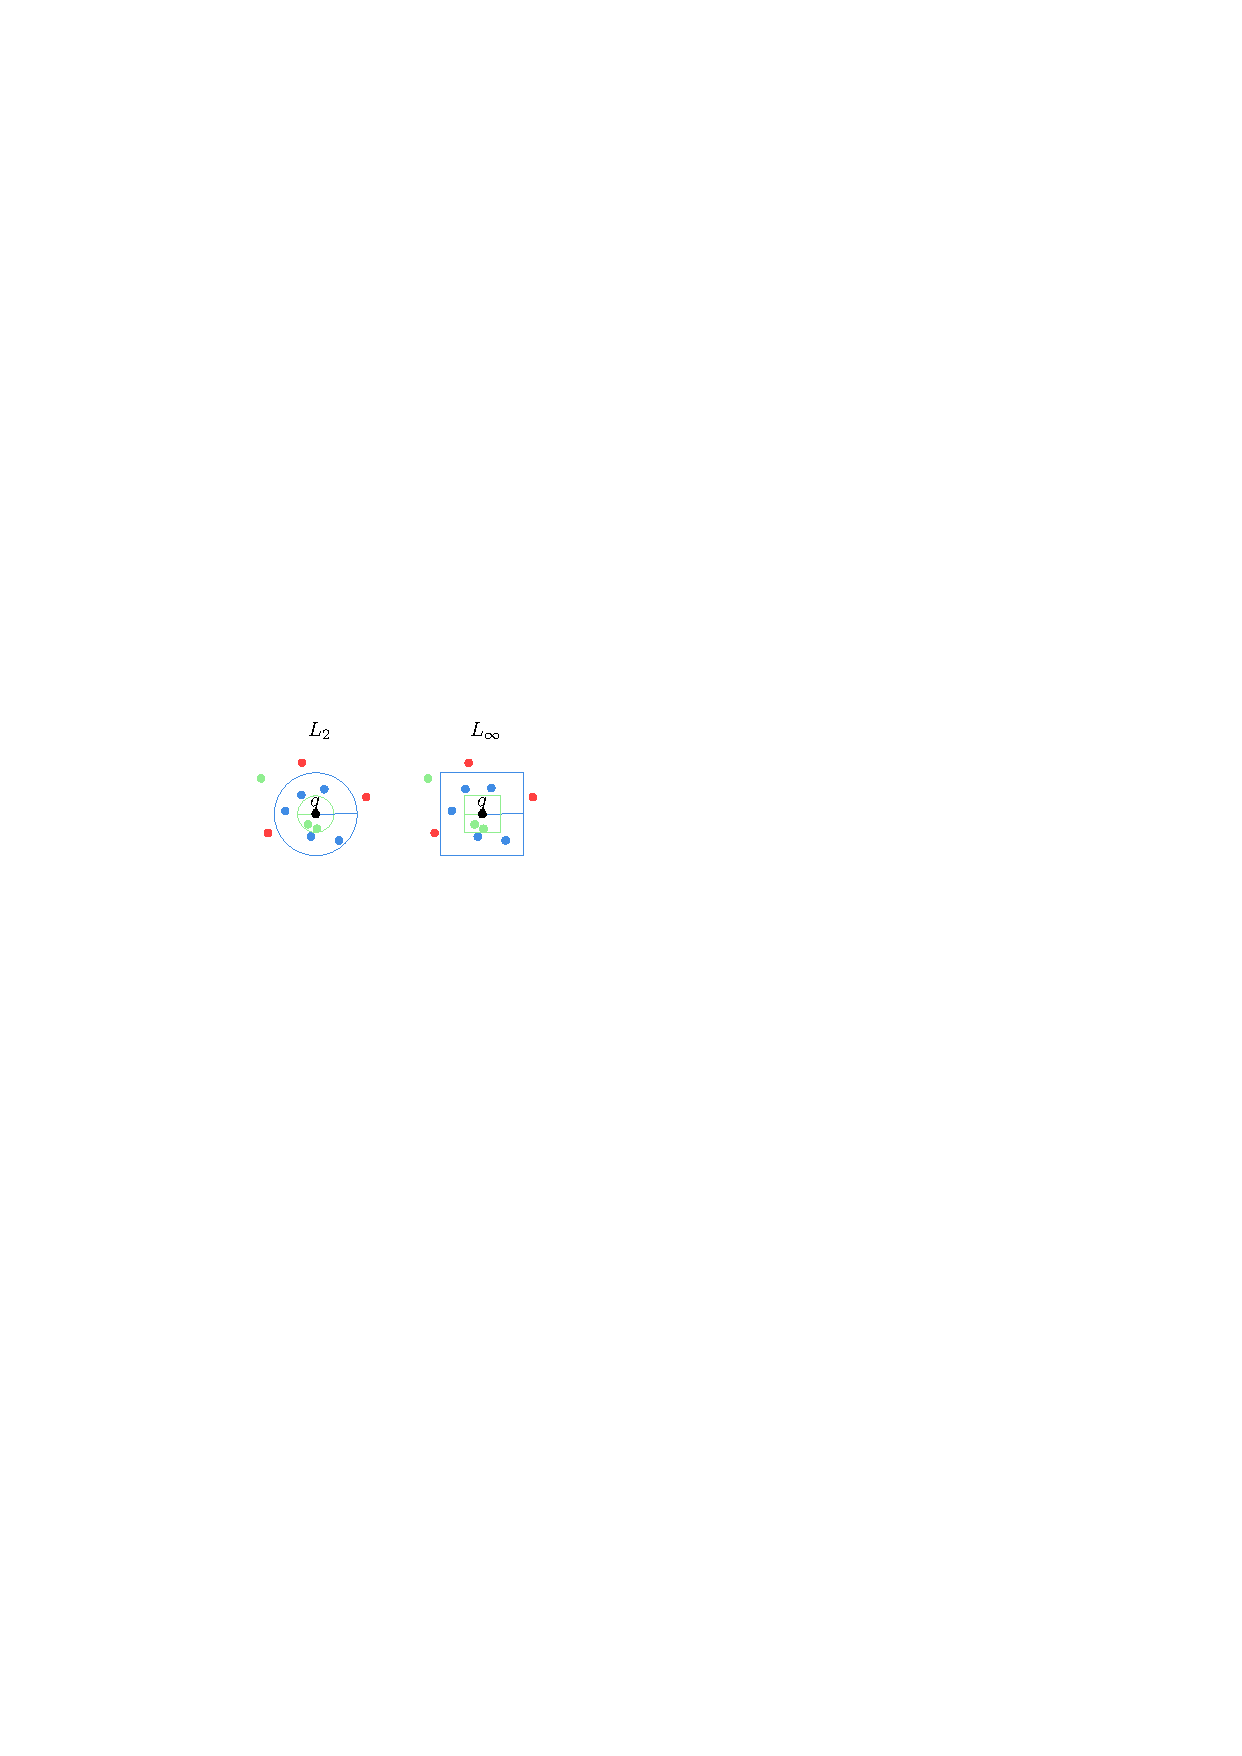
\includegraphics{figures/introFigure}
  \caption{A small colored point set and query point $q$; left with the $L_2$ distance measure, and right with the $L_\infty$ distance measure. For both $k = 2$ would yield green, while $k = 7$ yields blue.}
  \label{fig:introFigure}
\end{figure}


\subparagraph{The problem setting.}  We will consider one of the ``easiest''
settings for the data structures: points in $d=1$ and $d=2$ dimensions, and using
the $L_\infty(p,q) = \max_{i=1}^d |p_i-q_i|$ metric. If even
in these settings these data structures cannot out-perform more naive
strategies there seems little hope for more realistic scenarios
(higher dimensions and more general distance measures). The key
component in these data structures is a data structure for \emph{range
  mode queries}, that is, reporting the mode color among the points in
a query range. We actually show that combining ideas from both van
der Horst, Löffler, and Staals~\cite{chromatic_knn2025} and Chan
\etal~\cite{chan2014modeQuery} we obtain a simple $O(n)$ space data
structure, that can answer 2D range mode queries with axis aligned
squares ---and thus answer our chromatic $k$-NN queries with the
$L_\infty$ metric--- in $\tilde{O}(n^{2/3})$ time. This matches the
bound from van der Horst, Löffler, and Staals, but is arguably simpler
than their data structure. This approach generalizes to any constant
dimension $d$, and any distance measure whose unit disk is a constant complexity polytope, such as $L_1$. In our chosen setting, answering range mode queries is
related to answering type-2 color counting queries~\cite{gupta1995colorReporting,janardan1993generalizedIntersectionSearching,gupta2018ColoredSearchingSurvey},
computing heavy hitters~\cite{misra1982finding}, and answering top-$k$
queries~\cite{yu2012processing,rahul2011efficient}. Conceivably, our ideas may transfer to some of
these settings.

\subparagraph{Research Questions.} To answer our main research
question, determining how applicable these mode-finding data
structures are in practice, we identify several important
sub-questions:

\begin{enumerate}
\item Several of the data structures have sublinear query times like
  $O(n^{2/3})$. Hence, for sufficiently large $n$, $\phi$, and $k$, these data
  structures should outperform trivial solutions that count all colors, or even
  consider all points. For which values of
  $n$, $\phi$, and $k$ is this the case, and can we still efficiently construct the data
  structures for such values of $n$?

\item Most of the methods have parameters that govern the space and
  query time. Theory dictates an optimal choice of these
  parameters. Does this theoretical optimal choice of parameters
  correspond to the practical optimal choice?

\item In the analysis of algorithms we often focus only on obtaining
  worst case guarantees. However, it is unclear whether real world
  inputs display such worst-case behavior. Instead, the query time may
  depend on the specific input data. What happens when the colors are
  very strongly grouped, or very mixed? What happens when then number
  of colors is small, or very large?
\end{enumerate}

\subparagraph{Contributions.} Our experiments show that the more
complicated data structures indeed outperform more naive methods when $k$
(and $n$) are large in, on the data sets we performed our tests on. Additionally, in 1D our simpler data structure outperforms the more direct approach of Van der Horst, Löffler, and
Staals in query time, build time, and space usage, in practice. Hence,
this shows that developing a simpler solution may pay of
significantly, despite having the same asymptotical bounds! In terms of the dependency on the parameters, the results do not deviate much from what one would expect, both on synthetic and on real world data.

\subparagraph{Overview and organization.} We follow the approach from
van der Horst, L\"offler, and Staals~\cite{chromatic_knn2025}, who
observe that chromatic $k$-NN queries can be answered using two separate
queries:

\begin{description}
\item[a range finding query:] Given a query point $q$ and integer $k$,
  find a square $Q$ centered at $q$ that contains exactly $k$ points
  from $P$ (by finding the $k^\mathrm{th}$ furthest point
  $p_k \in P$), and
\item[a mode finding query:] Given a query square $Q$, compute the
  mode color of $P \cap Q$.
\end{description}

We thus build and implement separate data structures to answer these
queries. In \cref{sec:Range_finding} we briefly describe the
data structures for range finding queries. Answering a mode finding
query turns out to be much more challenging (and expensive), so the remainder of the article is mostly focused on answering such queries
efficiently. In particular, in \cref{sec:Mode_finding} we
review the data structures of Chan~\etal~\cite{chan2014modeQuery}
(\cref{sub:A_grid_based_data_structure}) and of van der Horst,
L\"offler, and Staals~\cite{chromatic_knn2025}
(\cref{sub:A_cutting_based_data_structure}). In
\cref{sec:The_grid_data_structure_for_queries_with_hypercubes},
we show that we can actually use a technique from the cutting-based data structure to
analyze the space usage of (a variation of) the grid based data
structure, thereby combining the best of both worlds. We present our
experimental setup ---including the implementation details, the
``naive'' reference methods, data sets, and the evaluation methods
that we use--- in \cref{sec:experimental_setup}. The results of
our experiments can be found in
\cref{sec:Experimental_Results}. Our code is available
at~\cite{code}.


\section{Mode finding.}
\label{sec:Mode_finding}

For the second subproblem we are given a query range (an interval in
1D, or a square in 2D), and wish to report the mode color among the
points contained in that range. The following (rephrased) observation
from Krizanc, Morin, and Smid~\cite{krizanc2005modeSets} is central:

\begin{lemma}[Krizanc, Morin, and Smid~\cite{krizanc2005modeSets}]
  \label{lem:modeColors}
Let $A$ and $B$ be multisets. If $c$ is a mode color of $A \cup B$, then either (i) $c \in A$, or (ii) $c$ is a mode of $B$, or both.
\end{lemma}

In Section~\ref{sub:A_grid_based_data_structure} we describe the grid-based method by
Chan \etal~\cite{chan2014modeQuery}. In Section~\ref{sub:A_cutting_based_data_structure} we
describe the cutting based approach of Van der Horst, Löffler, and
Staals~\cite{chromatic_knn2025}.


\subsection{A block based data structure.}
\label{sub:A_grid_based_data_structure}
We briefly review the block-based data structures by Chan \etal. We
start with the approach for $n$ points in $\R^1$.

\subparagraph{A block mode data structure.} Chan \etal give an $O(n)$
space data structure for points in $\R^1$ with $O(\sqrt{n / \log n})$
query time~\cite{chan2014modeQuery}; we will use a simpler version
with $O(\sqrt{n})$ query time instead (see Section 3
in~\cite{chan2014modeQuery}). W.l.o.g. we assume here the points have
unique integer coordinates in $\{ 0 \dots n-1 \}$. Let
$1 \leq s \leq n$ be an integer parameter. We then partition the
points into $s$ blocks numbered $1 \ldots s$, each containing $O(n/s)$
points. We store four arrays:

\begin{description}
\item[\texttt{blockModes} and \texttt{blockModeFrequencies}.] For each
  pair of blocks $1 \leq i \leq j \leq s$, consider the set of points $P_{i,j}$ in blocks $i$ through $j$. We store a mode color of $P_{i,j}$ as
  \texttt{blockModes[i,j]}, and its frequency as
  \texttt{blockModeFrequencies[i,j]}.
\item[\texttt{colorIndices}.] For each color $c$ we store a sorted array of the indices of all points of that color as\texttt{colorIndices[c]}.
\item[\texttt{rankInColor}.] For every point $i$ we store the rank of that point among its own color as \texttt{rankInColor[i]}.
\end{description}

See \cref{fig:1Dexample} for an example. Note that, for point $i$ of color $c$, \texttt{colorIndices[c][rankInColor[i]] = i}. 

\begin{figure}[tb]
  \centering
  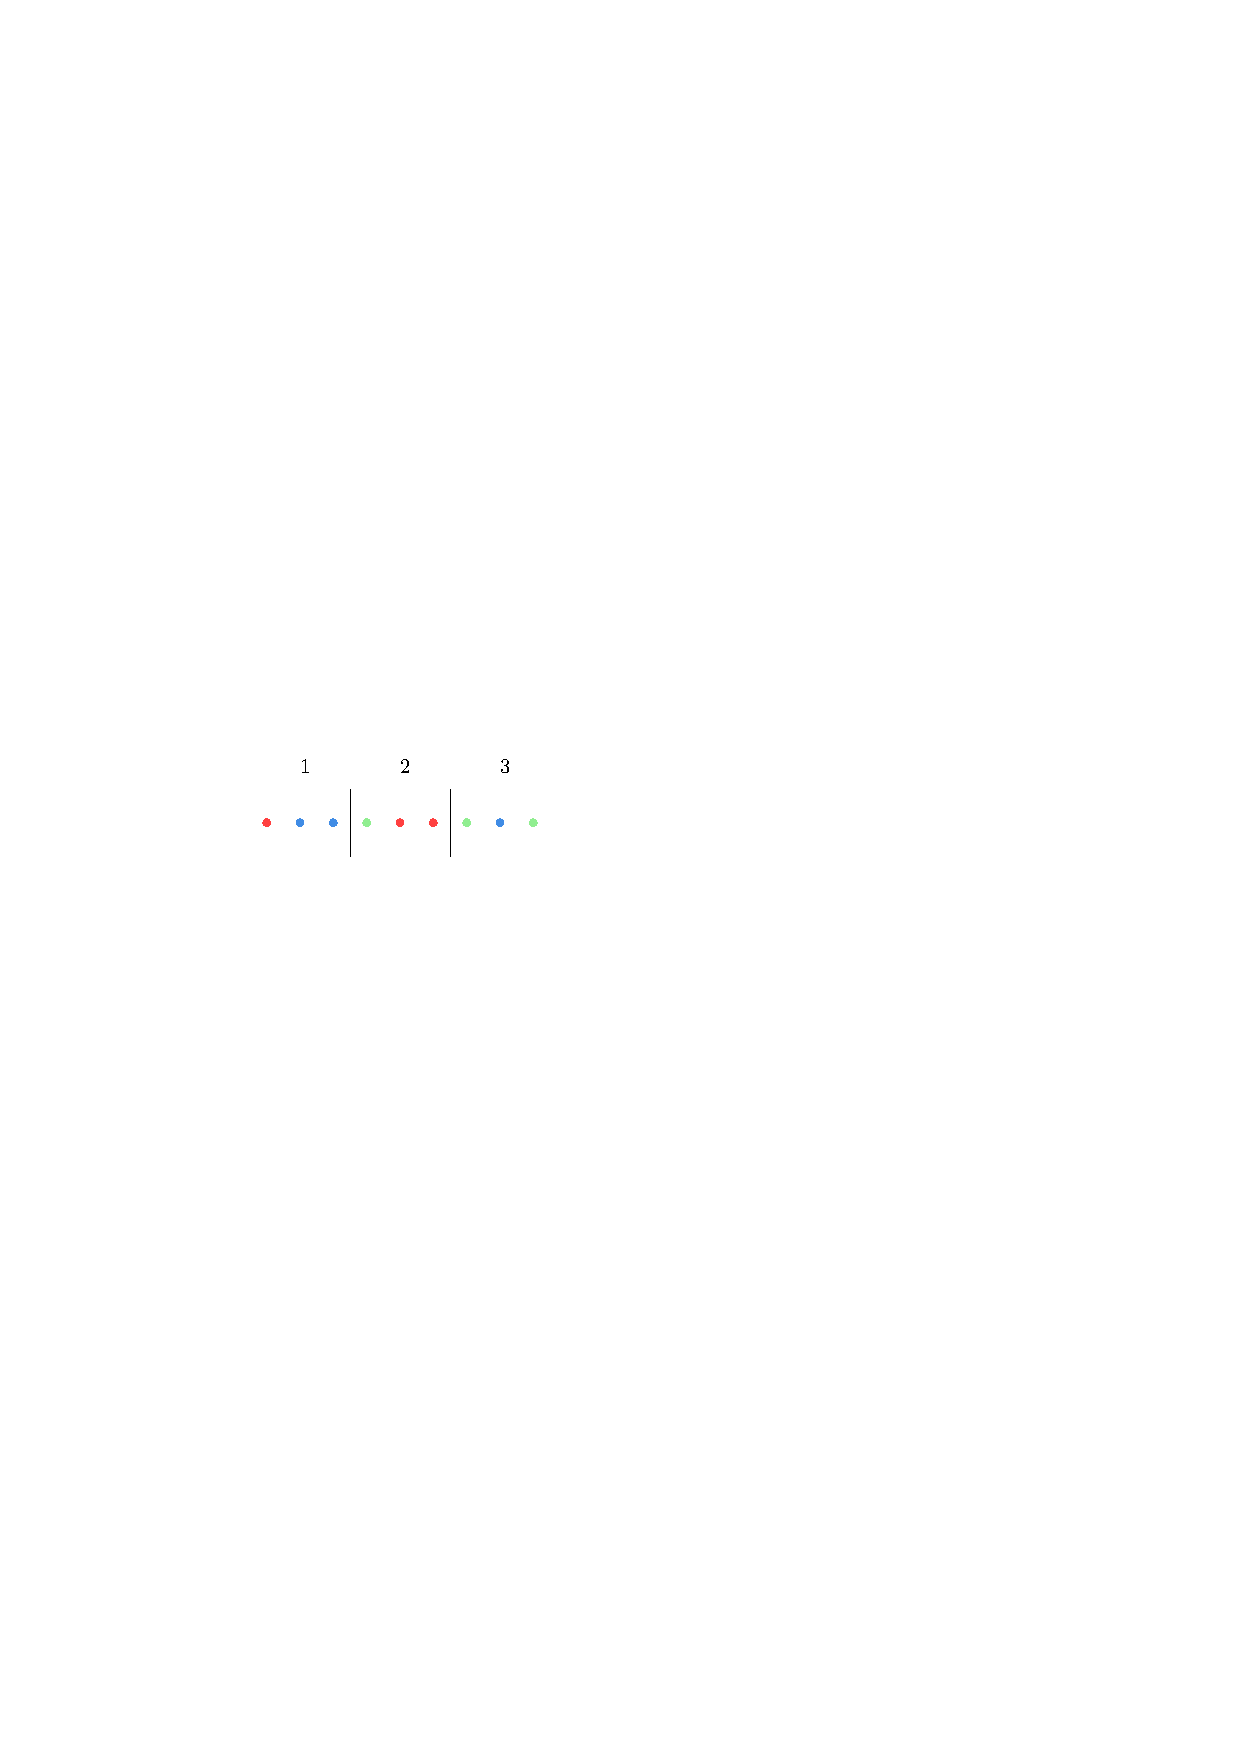
\includegraphics{figures/1Dexample}
  \caption{ An example set of $9$ points with $s = 3$ blocks; let $r,g,b$ be the colors red, green, and blue, respectively. Then
  $\texttt{blockModes} = \big[ \begin{smallmatrix} b & r & r \\ - & r & g \\ - & - & g \end{smallmatrix} \big] $,
  $\texttt{blockModeFrequencies} = \big[ \begin{smallmatrix} 2 & 3 & 3 \\ - & 2 & 3 \\ - & - & 2 \end{smallmatrix} \big] $,
  $\texttt{colorIndices[r]} = [ 0, 4, 5]$,
  $\texttt{colorIndices[g]} = [ 3, 6, 8]$,
  $\texttt{colorIndices[b]} = [ 1, 2, 7]$, and
  $\texttt{rankInColor} = [ 0, 0, 1, 0, 1, 2, 1, 2, 2]$.
  }
  \label{fig:1Dexample}
\end{figure}

The data structure uses $O(n + s^2)$ space, so we set $s = \sqrt{n}$
to use linear space. Construction takes $O(ns)$ time: $O(n)$ time for
\texttt{colorIndices} and \texttt{rankInColor} (using a simple scan),
and $O(ns)$ time for \texttt{blockMode}s (for a given block $i$ we can
compute \texttt{blockModes[i,j]} for all $j$ in $O(n \log n)$ time by
scanning from the start of block $i$ to the end of the array, while
maintaining the frequency of each color).

\subparagraph{Answering a query $[a,b]$.} We compute the blocks $i$ and
$j$ that contain $a$ and $b$ respectively. If $i = j$ we simply
iterate through the block and output the color with the largest
frequency. Otherwise, we can split the query in three (possibly empty)
parts: the \emph{prefix} from $a$ to the end of block $i$, the \emph{span} from
block $i+1$ through block $j-1$, and the \emph{postfix} from the start of
block $j$ to $b$. We first set the candidate mode color $c_m = \texttt{blockModes[i+1,j-1]}$ and
candidate frequency $f = \texttt{blockModeFrequencies[i+1,j-1]}$ to the
mode color and frequency of the span.
We then iterate through the prefix, from
left to right. Consider point $p$ of color $c$, with
$\texttt{rankInColor[p] = r}$. If we have already considered a point of
color $c$ (if $\texttt{colorIndices[c][r-1]} \geq a$) we skip
it. If not, we compute whether color $c$ has a larger frequency than the current
candidate mode color: this is the case if and only if $\texttt{colorIndices[c][r +
  f]} \leq b$ (i.e. if the next $f$ points of color $c$ all lie within
the range $[a,b]$). If so, we set $c$ as the new candidate mode
color, and compute its actual frequency by walking through
\texttt{colorIndices[c]} until we leave the range $[a,b]$, starting from \texttt{colorIndices[c][r + f]}.
We then proceed to the next point. We
similarly process the postfix, in reverse order. By \cref{lem:modeColors} at least one
of the considered colors must be a mode color of $[a,b]$. Since each
block contains $O(n/s)$ points, this takes $O(n/s)$ time in total.


\subsubsection{Extending to higher dimensions.} The above idea extends
to higher dimensions as well. Let $P$ be a set of $n$ colored points
in $\R^d$. We show how to answer range mode queries of the form
$Q=[a_1,b_1] \times [a_2,b_2] \times \cdots \times [a_d,b_d]$.

In each dimension we again partition the points into $s$ slabs using
$s-1$ parallel hyperplanes, such that there are $O(n/s)$ points in any
slab. This results in a $s \times s \times s \times \dots$ grid \G
with $s^d$ cells. For a query (hyper-)rectangle $Q$, the \emph{span}
generalizes to the the largest grid (hyper-) rectangle contained in
$Q$ whose sides lie on grid hyperplanes, and the \emph{pre- and
  postfix} generalize to the remaining parts of $Q$. See
Figure~\ref{fig:spanExample}.

\begin{figure}[tb]
  \centering
  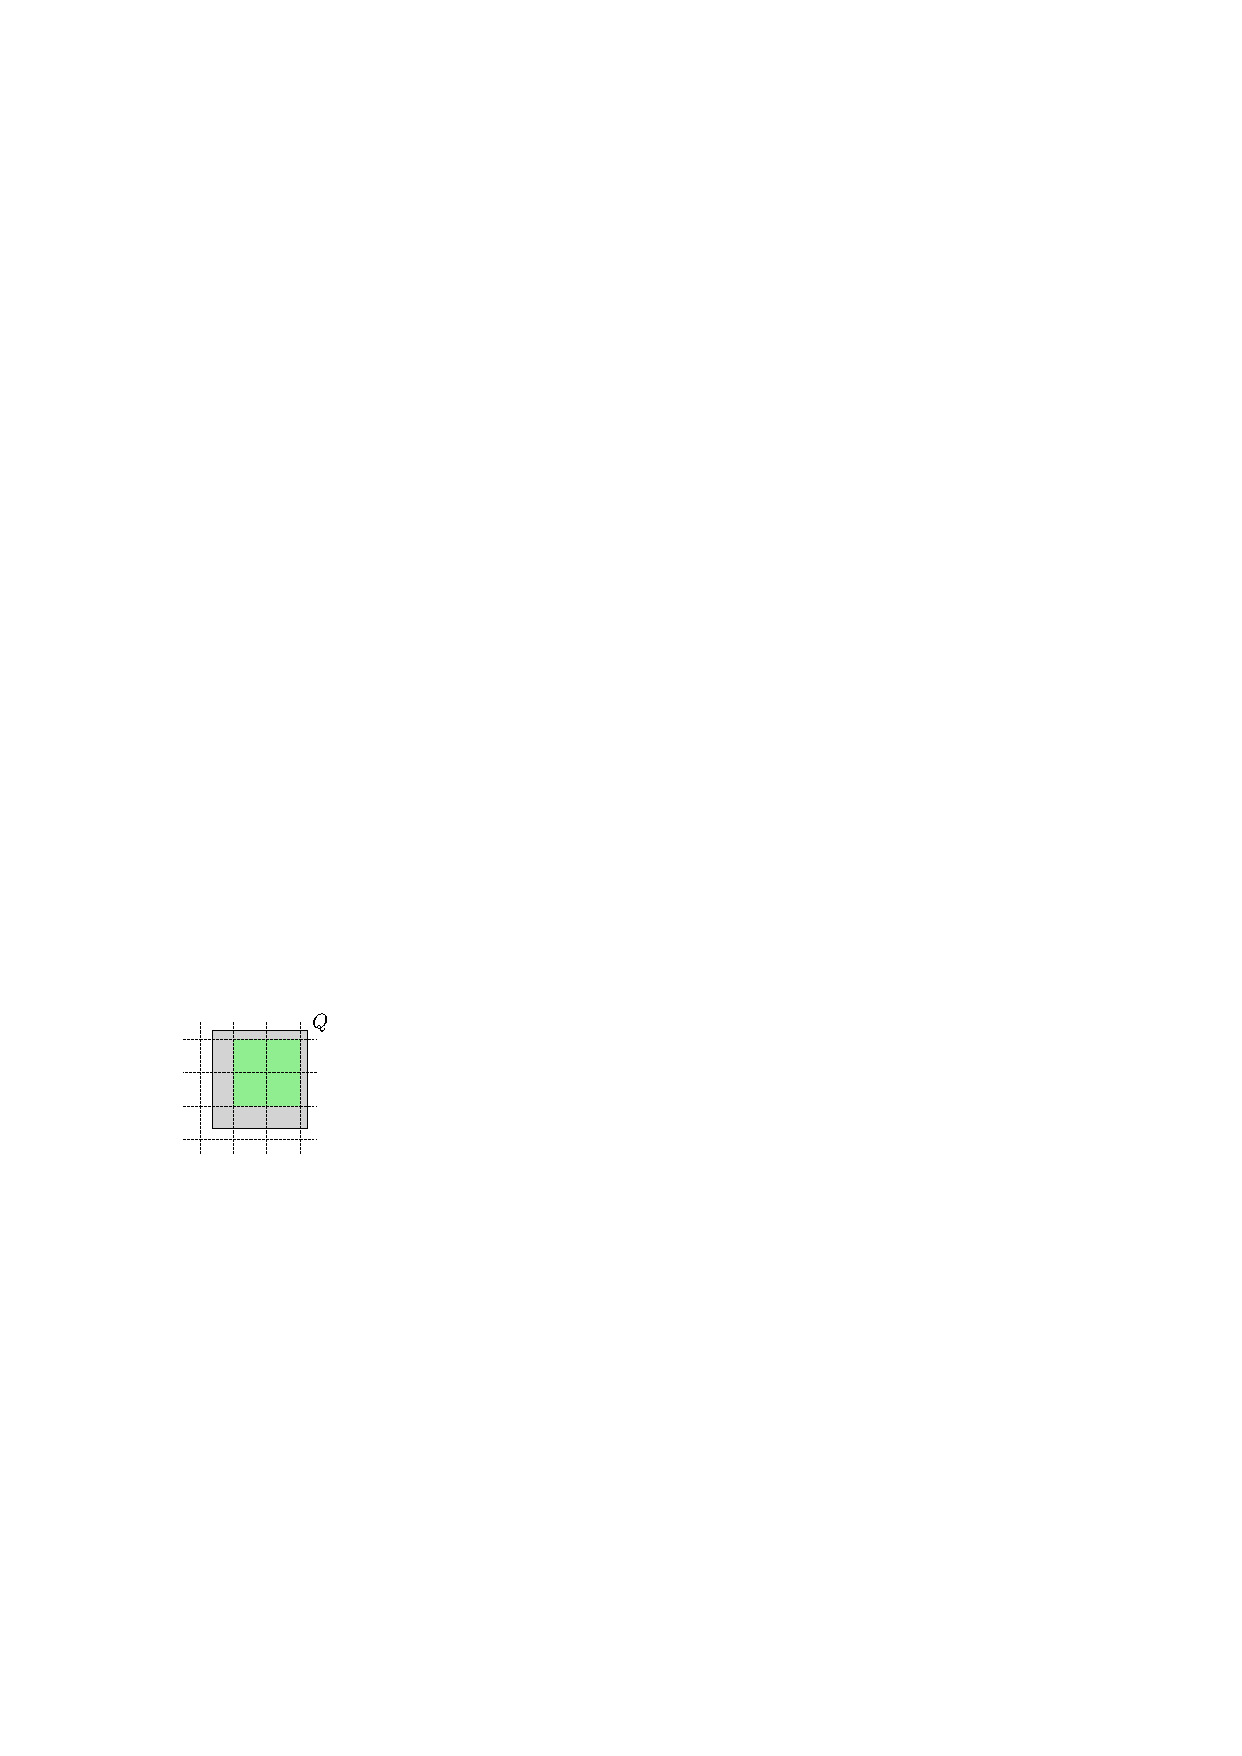
\includegraphics{figures/spanExample}
  \caption{ A query $Q$ with its span in green, and its generalized pre- and postfix in gray. }
  \label{fig:spanExample}
\end{figure}

\subparagraph{The data structure.}  For each distinct span we
precompute and store the mode color in a lookup table (accessed by the
indices of the minimum and maximum slab containing the span in each
dimension). Since there are $O(s^{2d})$ pairs of grid cells and thus $O(s^{2d})$ distinct spans, this uses $O(s^{2d})$ space. Additionally we build a range tree on the points of each color separately, of $O(n \log^{d-1} n)$ total size, for a total size of $O(s^{2d} + n \log^{d-1} n)$.

\subparagraph{Answering a query $Q$.} For each dimension, we find the
two slabs containing $Q$'s corners, by binary searching among the
hyperplanes. We iterate through all points in these slabs, and select the subset of them that is also contained in $Q$. Let $C$ be the set of their colors (similar to the pre- and postfix in
1D). Additionally we look up the mode color $c$ of the span of $Q$ in
our table, and add $c$ to $C$. Then for every color in $c \in C$ we
compute the frequency of $c$ in $Q$ using the range tree for color
$c$, and output the color with the highest frequency. By
\cref{lem:modeColors}, this color must be a mode color of $Q$. This
takes $O(\log n)$ time per color, and since each slab contains
$O(n/s)$ colors it takes $O((n/s)\log n)$ time in total.


\subsection{A cutting based data structure.}
\label{sub:A_cutting_based_data_structure}
We describe the approach of Van der Horst
\etal~\cite{chromatic_knn2025} to answer square mode queries in
$\R^2$.

Every square $Q$ is defined by a center point $(x,y)$ and a radius
$r$. Hence, a query square $Q$ corresponds to a point
$Q' = (x,y,r) \in \R^3$ (i.e. the parameter space $\R^3$ represents
all possible queries). See Figure~\ref{fig:thijsMethodPyramid}. We can
view this as a ``pyramid'' with $90\degree$ angles whose tip ends in
$Q'$; the intersection of this pyramid and the $(x,y)$-plane is
exactly $Q$. A point $p = (p_x,p_y)$ is contained in $Q$ if and only
if the point $(p_x,p_y,0)$ lies below the boundary of the
pyramid. Inversely, the set of squares containing $p$ form an ``upside
down pyramid'' $\nabla_p$ centered at $p$. We will consider $\nabla_p$
as (the graph of) a function. A square $Q' = (x,y,r)$ contains $p$ if
and only if $Q'$ lies above $\nabla_p$. Let
$F = \{\nabla_p \mid p \in P\}$ be the set of all these
functions. Given a query point $Q'$ (query square $Q$) we thus wish to
find the mode color among all points $p$ whose function $\nabla_p$
passes below $Q'$.

\begin{figure}[tb]
  \centering
  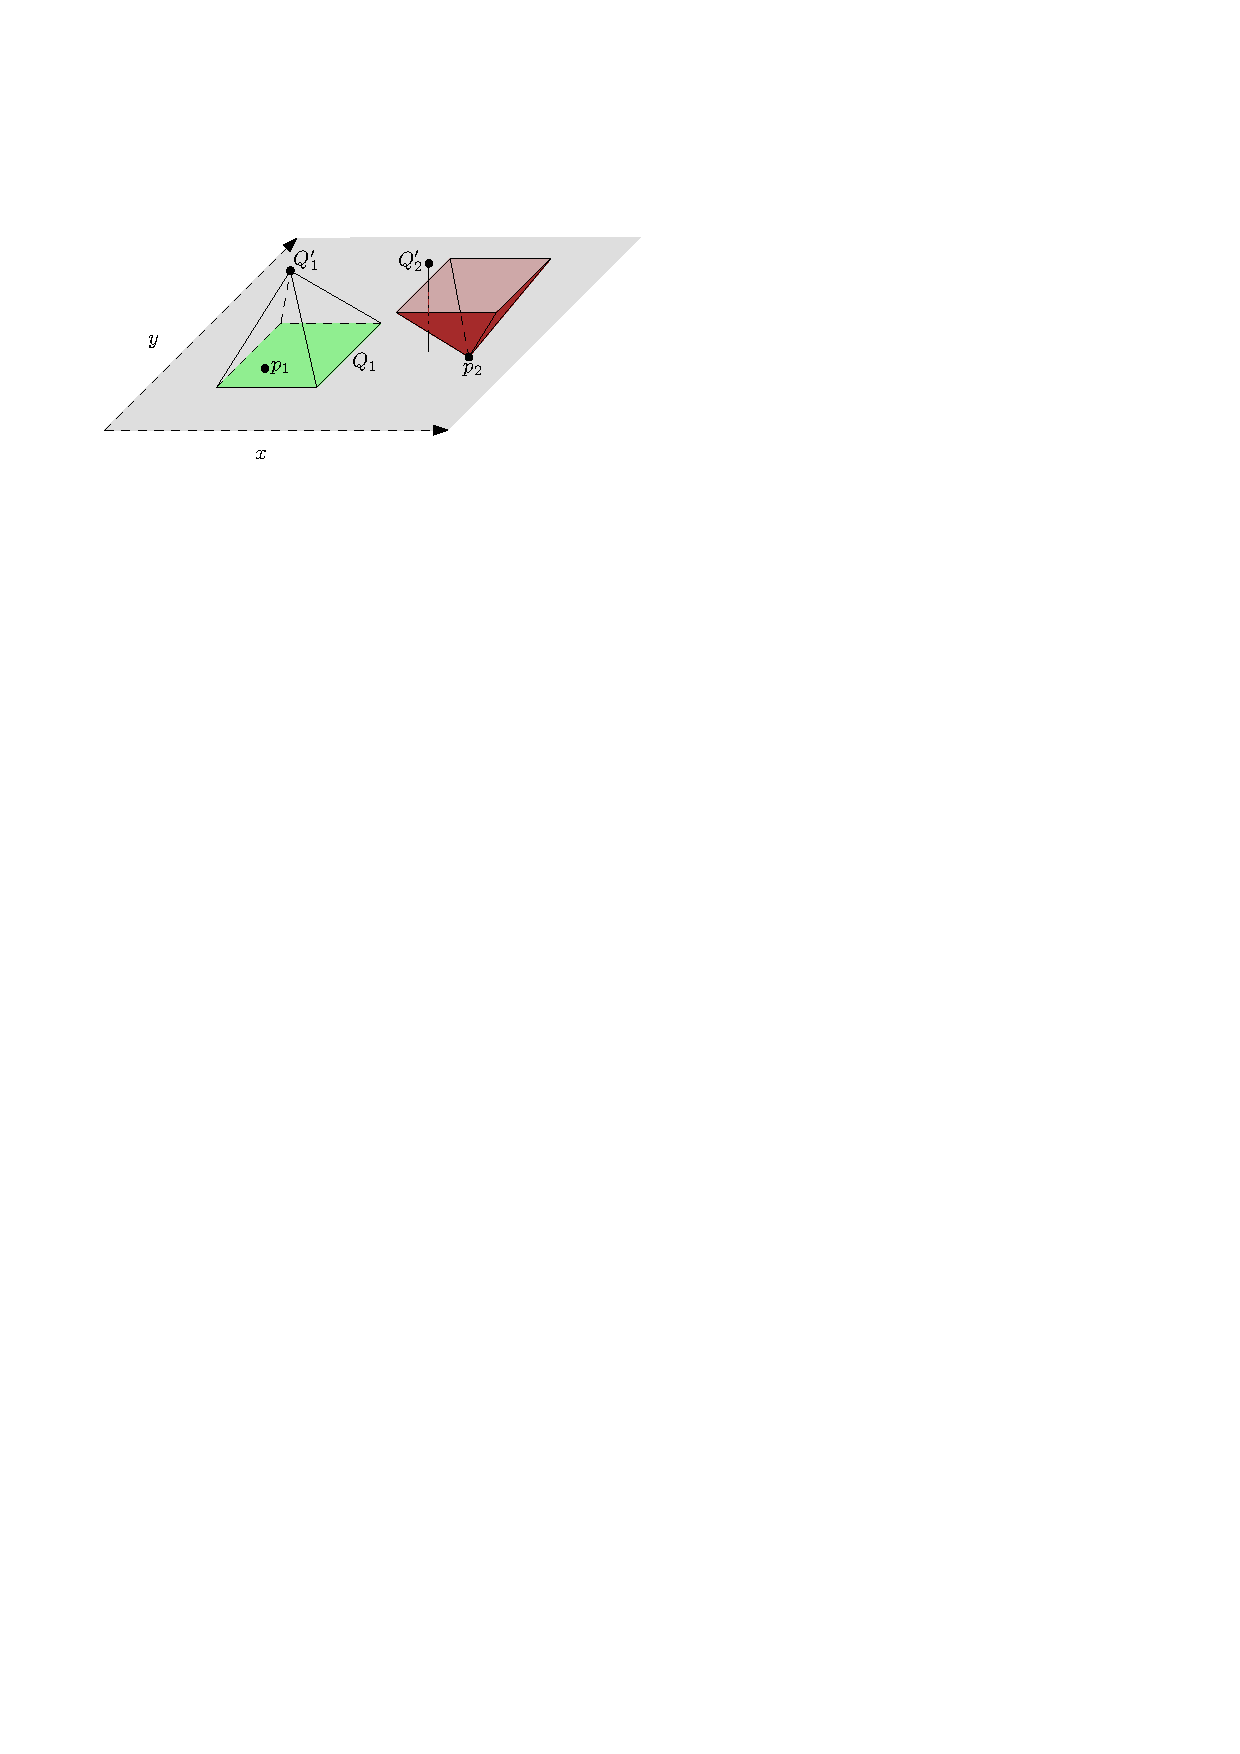
\includegraphics[width=\linewidth]{figures/thijsMethodPyramid}
  \caption{A pyramid formed by a square $Q_1$, and an upside down pyramid formed by a point $p_2$.
  }
  \label{fig:thijsMethodPyramid}
\end{figure}

\subparagraph{The data structure.}
A \emph{$(1/s)$-cutting $\Xi$ of $F$} is a subdivision of $\R^3$ into constant complexity cells,
so that each cell $\Delta \in \Xi$ is intersected by at most $n/s$ functions from $F$.
Let $F_\Delta \subseteq F$ denote the subset of functions that
intersect (the interior of) $\Delta$; i.e. the \emph{conflict list} of $\Delta$. We compute and store a $(1/s)$-cutting $\Xi$ of $F$
with $O(s^3)$ cells~\cite{chazelle1993cutting}. For each cell $\Delta$ we compute the mode color $c_{\Delta}$ of all functions
passing below $\Delta$ (and its frequency). Additionally, we build a data structure that can
quickly report the conflict list of a given cell.
For every color $c$ we also build a range tree on all points of color $c$
that can answer counting queries. The data structure has size $O(n \log n + s^3)$ and can be built in $O(n \log n + r^3 \log n + nr^2)$ time.

\subparagraph{Answering a query $Q' = (x,y,r)$.} We first locate the cell $\Delta$ containing $Q'$.
By \cref{lem:modeColors}, either $c_{\Delta}$ or some color in $F_\Delta$ must be a mode color for $Q'$.
Thus, for each of these colors separately we perform a range counting query. Since the conflict list has size $O(n/s)$, this takes $O((n/s)\log n)$ time. We report the color with the highest frequency.


\subparagraph{Adaptation for $\R^1$.}
The above technique for answering mode queries in $\R^2$ can be
simplified to work for queries in $\R^1$. Now, a query can be
parameterized by midpoint $x$ and radius $r$, so $\R^2$ represents all
possible queries $Q = (x,r)$. The function $\nabla_p$ of a point $p$
is now ``v-shaped'', and there exists a cutting of all these functions
with $O(s^2)$ cells. Answering a query is analogous to the
version in $\R^2$.


\section{The grid data structure for range mode queries with  \texorpdfstring{$L_{\infty}$}{L∞} disks.}
\label{sec:The_grid_data_structure_for_queries_with_hypercubes}
In this section we first present a data structure that can answer queries under the $L_{\infty}$ distance metric, by combining ideas from both the block-based and the cutting-based methods. We later show how to extend this to other metrics such as $L_1$.

The grid based data structure from
\cref{sub:A_grid_based_data_structure} can answer queries with
arbitrary axis-aligned orthogonal boxes. However, to answer chromatic
$k$-NN queries in the $L_\infty$ distance, it suffices to
answer queries whose boxes that have equal side-lengths; that is,
hypercubes. Although there are $\Theta(s^{2d})$ possible combinatorially
distinct rectangular spans (and thus the blocks data structure uses
$\Theta(n \log^{d-1} n + s^{2d})$ space), not all of these can
actually be the span of a hypercube query; see
\cref{fig:simplifiedConstructionGridNoSquare}. We formalise this below.

Let a \emph{square span} be such a grid-rectangle whose sides lie on grid hyperplanes
that can be the span of a hypercube. Next, we will show that
only $O(s^{d+1})$ such square spans exist, by borrowing
some of the ideas that were used in the data structure
of~\cref{sub:A_cutting_based_data_structure}. Hence, we will compute
and store the mode color only for spans that correspond to hypercubes
(using e.g. a binary search tree or a hash table). This thus reduces the space used by the data structure to
$O(n \log^{d-1} n + s^{d+1})$. Furthermore, we will argue we can construct the data
structure in $O(n \log^{d-1} n + ns^d)$ time. Hence, this version of the grid based
method matches the performance of the more complicated cutting-based structure
from~\cref{sub:A_cutting_based_data_structure}; in fact, it can be seen as an alternate (and in our opinion simpler) description of the same data structure.

\begin{figure}[tb]
  \centering
  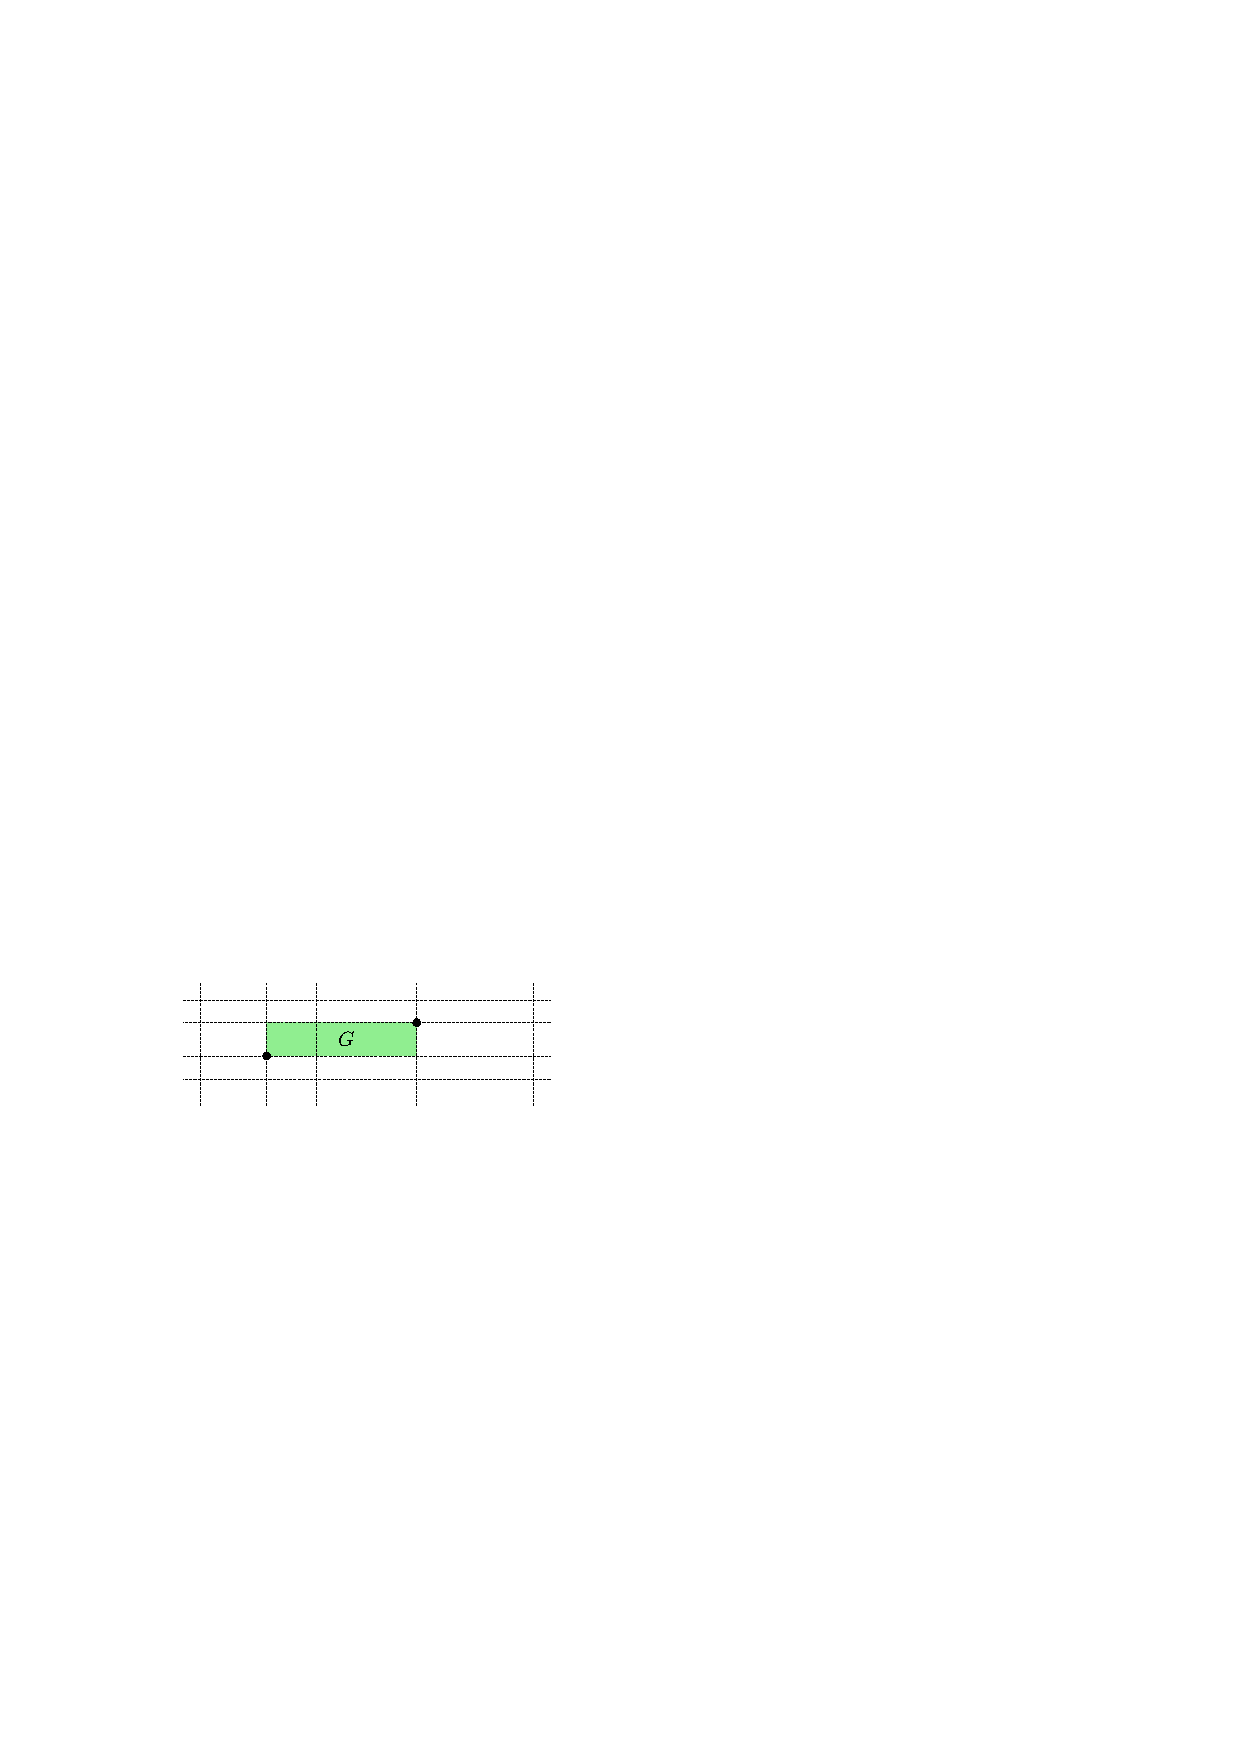
\includegraphics{figures/simplifiedConstructionGridNoSquare}
  \caption{There is no square for which $G$ is the largest grid-rectangle contained in it.}
  \label{fig:simplifiedConstructionGridNoSquare}
\end{figure}


\begin{figure}[tb]
  \centering
  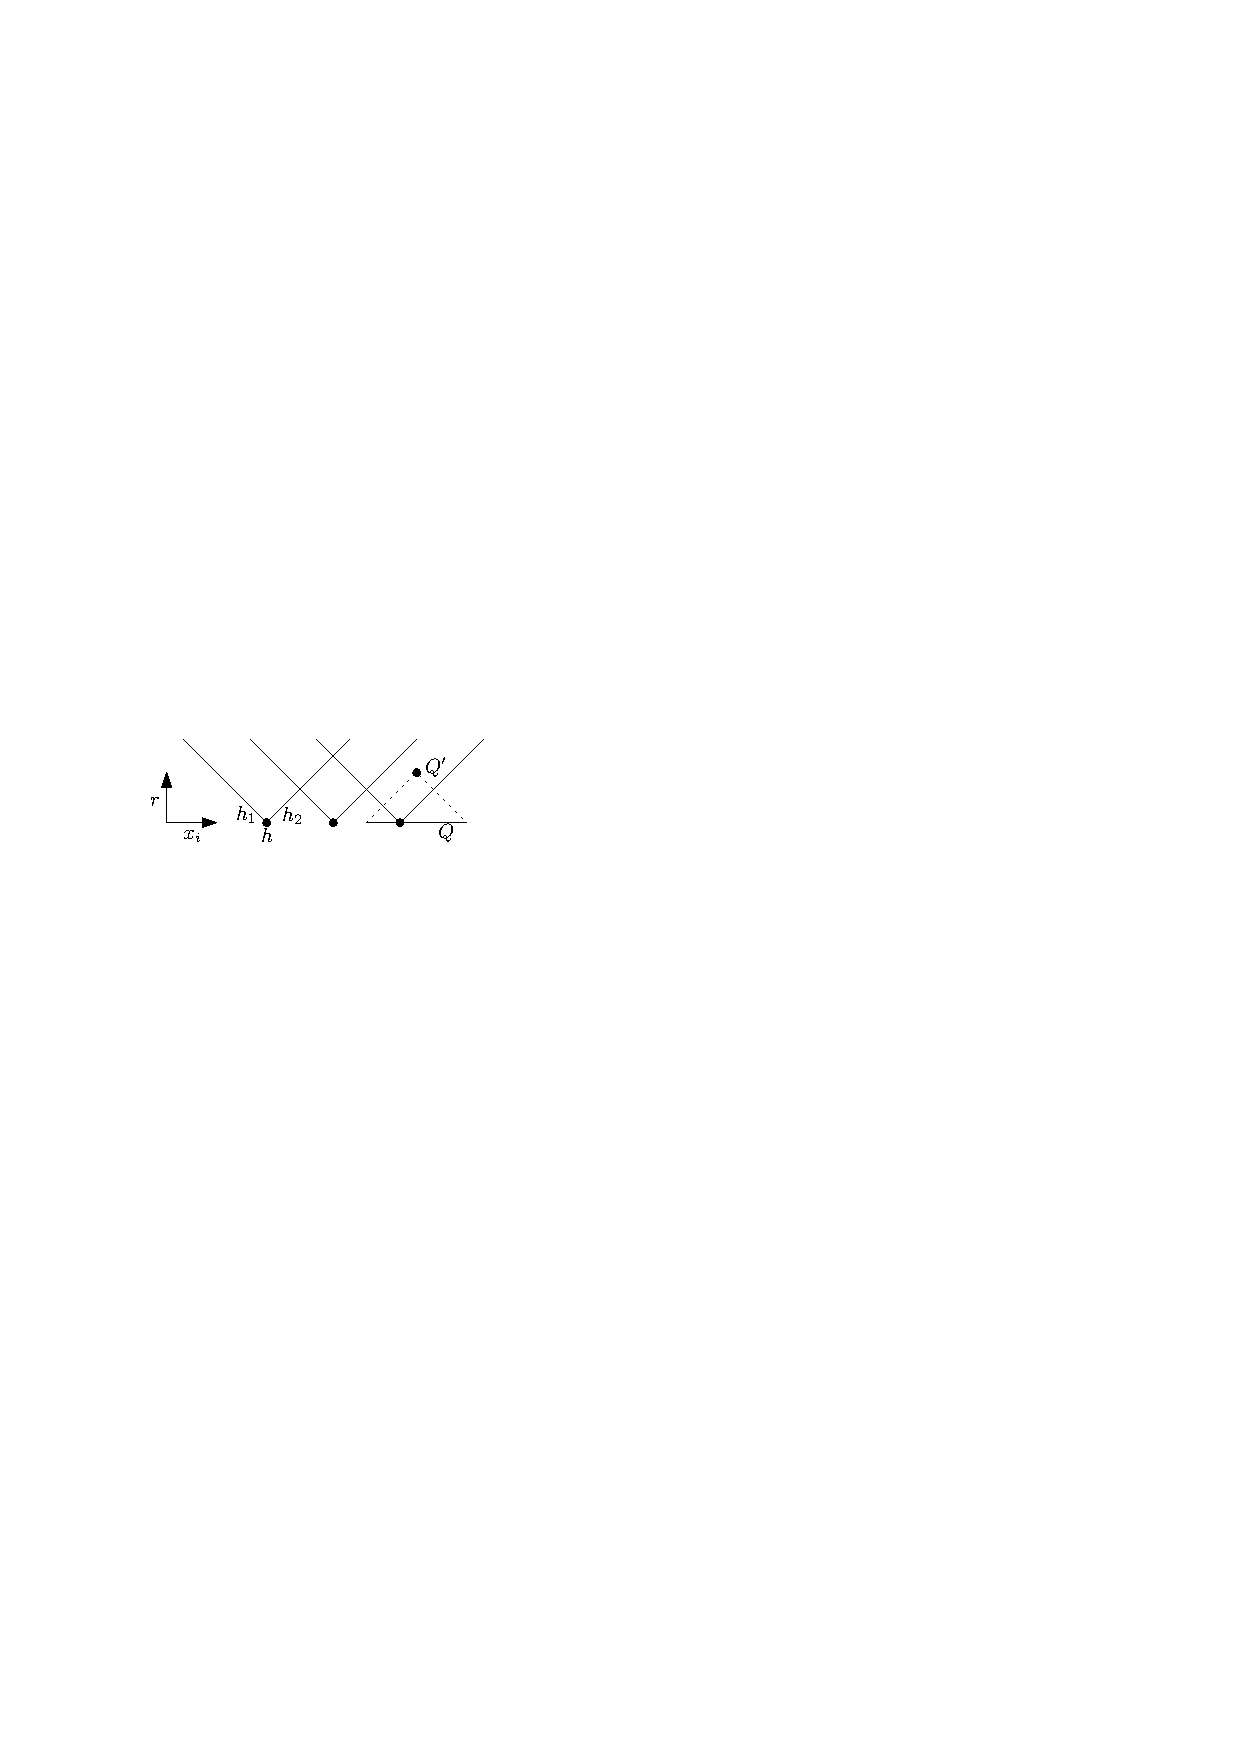
\includegraphics{figures/fewSquareSpans}
  \caption{A $d$-dimensional grid hyperplane $h: x_i = a$ creates two
    $(d+1)$-dimensional hyperplanes $h_1,h_2$. A square $Q$ intersects
    $h$ if and only if its corresponding point $Q'$ lies above $h_1$
    and $h_2$.}
  \label{fig:fewSquareSpans}
\end{figure}


\subparagraph{Reducing the space usage.} Consider the grid \G from
\cref{sub:A_grid_based_data_structure} that partitions $\R^d$ into
$s^d$ grid cells using $d(s-1)$ hyperplanes. As in
Section~\ref{sub:A_cutting_based_data_structure} we embed this grid on
the plane $r=0$ in a $d+1$-dimensional space (where $r$ denotes the
additional ($d+1^\mathrm{th}$) coordinate). For each $d$-dimensional
grid hyperplane $h: x_i = a$ we create two $(d+1)$-dimensional
hyperplanes $h_1: r = a - x_i$ and $h_2: r = -a + x_i$. See
\cref{fig:fewSquareSpans} for an illustration. Let $H$ be the set of
all $2d(s-1)$ of these $(d+1)$-dimensional hyperplanes that we create this
way. A square $Q$ centered at $(Q_1,\dots,Q_d)$ with radius $Q_r$
intersects the grid hyperplane $h$ if and only if $Q_i + Q_r \geq a$
and $Q_i - Q_r \leq a$, which happens if and only if
$Q' = (Q_1,\dots,Q_d,Q_r)$ lies above both $h_1$ and $h_2$.

Consider the arrangement \A of all $O(s)$ hyperplanes in $H$, which has
complexity
$O(s^{d+1})$~\cite{edelsbrunner86const_arran_lines_hyper_applic}.  All
$(d+1)$-dimensional points within one cell of the arrangement are
indistinguishable w.r.t. the hyperplanes in $H$.  That means their
corresponding squares intersect the same grid-hyperplanes, and thus
have the same span.  It follows that there are only $O(s^{d+1})$
distinct spans of square queries in the grid.

\subparagraph{Preprocessing.} Each cell in the arrangement \A
corresponds to a $d$-dimensional square span. Consider two adjacent
cells in \A, and observe that they are combinatorically equivalent
w.r.t. the $d+1$-dimensional hyperplanes, except the one dividing
them. It follows that their corresponding spans are equivalent
w.r.t. the $d$-dimensional hyperplanes defining the grid, except for
at most one slab in one dimension.

Hence, we will traverse the cells of \A (using e.g. a depth first
search) while maintaining the frequency of every color in the span
corresponding to the current cell. After every step we store the
current mode color with this current slab in the lookup table.  Since
two adjacent spans differ by at most one slab, which contains $O(n/s)$
points, we can update these frequencies in $O(n/s)$ time per
step (see Secttion 4.3 in~\cite{chromatic_knn2025} for why these updates can be performed in $O(1)$ time per step), or $O(ns^d)$ time in total for all $O(s^{d+1})$
cells. Note that it is not even needed to explicitly construct \A as
it itself has a grid-like structure: all the $h_1$ hyperplanes for the
grid lines of some coordinate $x_i$ are parallel, and appear in the
same order as the grid hyperplanes. Hence, it suffices to compute
these $2d$ sorted lists of these hyperplanes, and keep track of the
indices corresponding to the current cell of \A.


\subparagraph{Other distance metrics.} The above technique can also be
used for other distance metrics whose unit disk is a
constant-complexity convex polytope, for example $L_1$. The main idea
is that we can still define an irregular grid, and argue that the
number of grid cells that define queries is small. See
\cref{fig:constantComplexityUnitDisk} for an illustration, and see \cref{app:Omitted_Proofs} for the proof. In
particular, we obtain the following result:

\begin{figure}[tb]
  \centering
  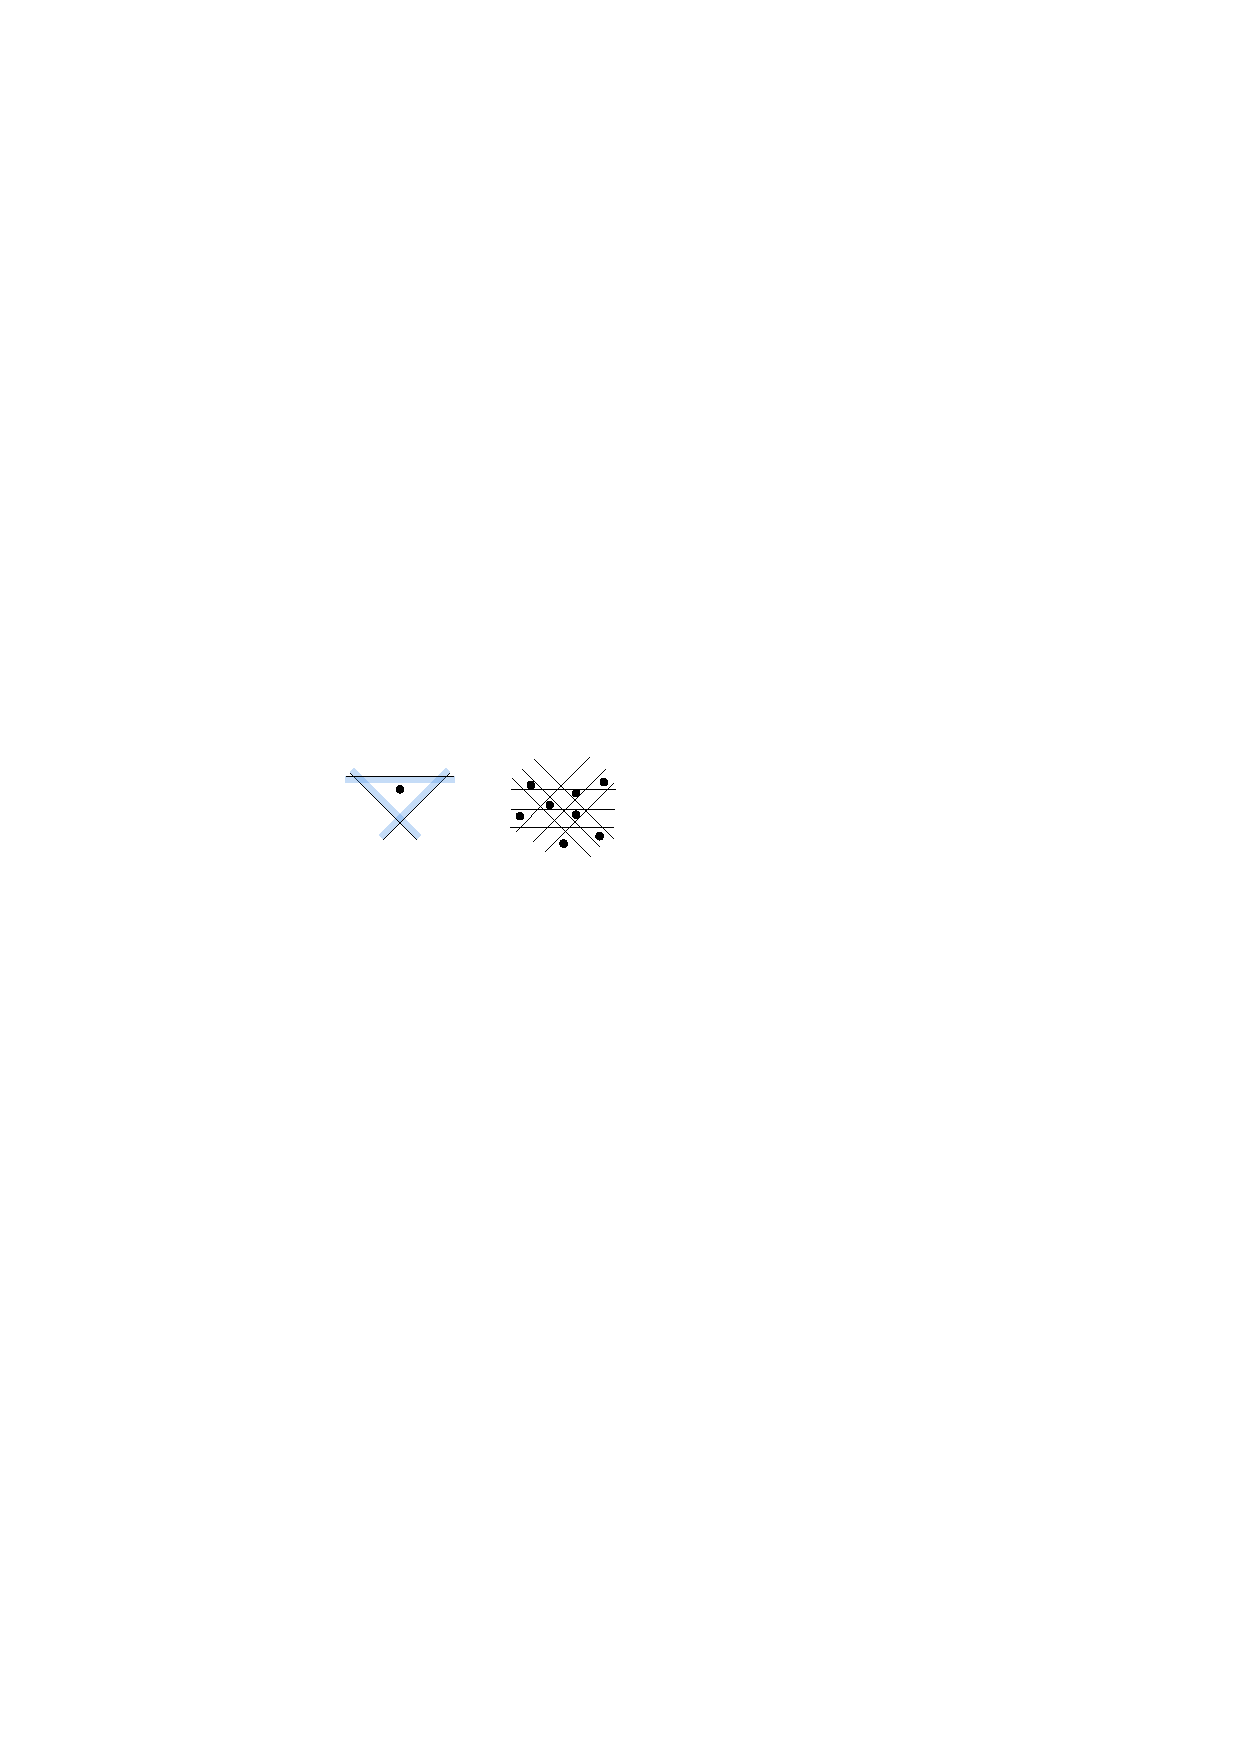
\includegraphics{figures/constantComplexityUnitDisk}
  \caption{A triangle unit disk in $\R^2$ that is the intersection of
    three halfspaces, and the irregular grid based on this unit disk
    where each strip contains two points.}
  \label{fig:constantComplexityUnitDisk}
\end{figure}

\begin{restatable}{theorem}{gridforCubes}
  \label{thm:grid_for_cubes}
Let $\hat{L}$ be a distance metric whose unit disk is a constant-complexity convex polytope. Given a set of points in $\R^d$ and a parameter $s$ we can build a data structure of size $O(n \log^{d-1} n + s^{d+1})$ in
  $O(n \log^{d-1} n + ns^d)$ time. Given a query point $q \in \R^d$ and radius $r \in \R$ it can report the mode color of all points at distance at most $r$ from $q$, according to $\hat{L}$, in $O((n/s)\log^{d-1} n)$ time.
\end{restatable}

This bound matches that of Van der Horst, Löffler, and
Staals; specifically, choosing $s = (n\log^{d-1}n)^{1/(d+1)}$ yields an $O(n \log^{d-1} n)$ space datastructure with query time $O((n \log^{d-1} n)^{1 - 1/(d+1)})$~\cite{chromatic_knn2025} (see Lemma 23, and Theorem 45). Similar to Van der Horst, Löffler, and Staals, we can also adapt this to a version using $O(n)$ space (by using high fanout range trees), using slightly more preprocessing and query time; see their article for details.


\section{Experimental setup.}
\label{sec:experimental_setup}
We experimentally test and compare several data structures for mode
finding. The data
structures were implemented in \cpp. The code and experimental results are available at~\cite{code}. \todo{publish code properly}

To answer 2D mode finding queries, the cutting-based datastructure from
\cref{sub:A_cutting_based_data_structure} would require building 3D
arrangements with point location. To our knowledge, these are unfortunately not readily
available in any widely used computational geometry library
(and would be a large amount of work to implement from scratch). Instead, we
implement the cutting-based datastructure for 1D queries; this uses 2D
arrangements, which are supported by The Computational Geometry
Algorithms Library (CGAL)~\cite{cgal:library,cgal:arrangements}.
We compare the 1D cutting-based structure to other 1D mode finding datastructures. If the cutting-based structure performs worse than the alternatives even in 1D, there is little hope that it will do better in higher dimensions.


\subsection{Implemented mode finding data structures.}
\label{sub:implementedDatastructs}

See \cref{tab:theoreticalOverview} for an overview of the worst case space usage and query times.

Both in 1D and in 2D we implement the following data structures:

\newcommand{\report}{\texttt{report}\xspace}
\newcommand{\rangeTrees}{\texttt{rangeTrees}\xspace}
\newcommand{\grid}{\texttt{grid}\xspace}
\begin{description}
    \item[1D/2D-\report] report all points within the query square using a range tree, and iterate through them while maintaining counts.
    \item[1D/2D-\rangeTrees] query the frequency of all $\phi$ colors separately (using a range tree per color).
    \item[1D/2D-\grid] the data structure described as described in \cref{sec:The_grid_data_structure_for_queries_with_hypercubes}
\end{description}

\newcommand{\blocks}{\texttt{blocks}\xspace}
\newcommand{\cutting}{\texttt{cutting}\xspace}
In 1D we have additionally implemented the following data structures:
\begin{description}
  \item[1D-\blocks] using the approach of Chan \etal~\cite{chan2014modeQuery} described in \cref{sub:A_grid_based_data_structure}.
  \item[1D-\cutting] using the approach of van der Horst~\cite{chromatic_knn2025} described in \cref{sub:A_cutting_based_data_structure}.
\end{description}


\begin{table}
  \centering
\begin{tabular}{lll}
\toprule
Structure  & Space               & Query time       \\
\midrule
1D \report     & $O(n)$              & $O(\log n + k)$  \\
1D \rangeTrees & $O(n)$              & $O(\phi \log n)$ \\
1D \blocks     & $O(n + s^2)$        & $O(n/s)$         \\
1D \cutting    & $O(n \log n + s^2)$ & $O((n/s) \log n)$  \\
1D \grid       & $O(n \log n + s^2)$ & $O((n/s) \log n)$  \\
2D \report     & $O(n \log n)$       & $O(\log^2 n + k)$  \\
2D \rangeTrees & $O(n \log n)$       & $O(\phi \log^2 n)$ \\
2D \grid       & $O(n \log n + s^3)$ & $O((n/s) \log^2 n)$  \\
\bottomrule
\end{tabular}
\caption{The worst case space usage and query times of the different
  implemented methods.}
\label{tab:theoreticalOverview}
\end{table}


\subsection{Implemented range finding data structures.}
\label{sec:Range_finding}
Although the focus of this research is on the structures for mode finding queries, a full $k$NN query also consists of a range finding query, where we are given a query point $q$ and an integer
$k$, and wish to compute the radius of a square centered at
$q$ that contains exactly $k$ points. Van der
Horst, Löffler, and Staals~\cite{chromatic_knn2025} present a structure in 1D with $O(\log n)$ query time using $O(n)$ space, and in 2D with $O(\log^2 n)$ query time using $O(n \log n)$ space. For simplicity, we instead implement the $O(\log^2 n)$ technique both for 1D and 2D queries, since the range finding queries are much faster than the mode finding queries anyway. We describe the technique for 2D; it trivially applies to 1D as well.

We build a range tree on all points that can answer rectangle
counting queries. Consider all points with smaller $x$-coordinate than
$q$; we will perform a binary search on these points. Given the point
$p$ with median $x$-coordinate among these points, we construct the
square centered at $q$ with radius $|q_x - p_x|$, and query the number
of points contained in this square. If this square contains less than
$k$ points we are looking for a larger square, so we recurse on the
points left of $p$ (= further away from $q$). If the square contains more than $k$ points we
recurse on the points right of $p$ (= closer to $q$). If the square
contains exactly $k$ points we are done. If this binary search
terminates and we have not yet found a square containing exactly $k$
points we repeat a similar procedure on all points with larger
$x$-coordinate, and then do the same for the $y$-coordinates. This
uses $O(n \log n)$ space for the range tree, and a query is answered
using $O(\log n)$ range-counting queries, in $O(\log^2 n)$ total time.



\subsection{Measurements.}
For each datastructure we measure the space usage, the preprocessing time, and the average query time. We measure these quantities as follows.
\begin{description}
  \item[Preprocessing and query time.] We measure time using \texttt{std::chrono::high\_resolution\_clock}, just before and after building the datastructure or performing the query. This reports so called ``wall-clock'' time in nanoseconds ($10^{-9}$ seconds). For queries, we first perform $\num{1000}$ and discard their result (since the earliest queries might be slightly slower due to caching) and then take the average time over $\num{10000}$ queries to minimize fluctuations and randomness.
  \item[Space usage.]  We measure space ``manually'', by counting the
    number of bytes required to store all the primitive types present
    in a data structure. For example, a vector that stores $10$
    \texttt{int}s of $4$ bytes each uses $10 * 4 = 40$ bytes of space.
    Additionally, the \cutting data structure contains a more
    complicated data structure, namely the
    \texttt{CGAL::Arrangement\_2} (and accompanying
    \texttt{CGAL::Arr\_trapezoid\_ric\_point\_location}) object. For
    an arrangement with $v$ vertices, $e$ edges, and $f$ faces we
    estimate the space usage assuming that it is implemented using a
    very basic DCEL, containing three edge-pointers per edge (next,
    twin, previous), and one edge pointer per vertex and face. The
    space usage computed this way can be an under-estimate of the real
    space usage, as we ignore any overhead such as allocated but
    unused space, or auxiliary pointers. This mostly affects the
    \cutting structure, which may thus use more space in
    practice. However, as we will see in
    Section~\ref{sec:Experimental_Results}, even with this
    under-estimate the \cutting structure uses \emph{more} space than
    the other data structures considered.
\end{description}


\subsection{Data sets.}
We use the following data sets in our evaluation.

\begin{description}
  \item[Synthetic uniform random data.] Given parameters $n$ and $\phi$, we generate $n$ points, uniformly sampled within a $10000$-radius cube centered at the origin, each with a color from $1 \dots \phi$, also uniformly at random. See \cref{fig:groupedVsUniform}.
  \item[Synthetic grouped data.] Given parameters $n$, $\phi$, $\alpha \in [0,1]$, and $\gamma \in \{0 \dots n\}$, we generate $n$ points, uniformly sampled within a cube. We pick $\gamma$ of them as \emph{center points}, and give them a color from $1 \dots \phi$, uniformly at random. For each of the remaining points, with probability $\alpha$ we set its color to that of the closest center point, and with probability $1 - \alpha$ we choose a color uniformly at random. The larger the value of $\alpha$, the stronger the grouping in the produced coloring.
  Specifically, with $\alpha = 0$ this is equivalent to the uniform random coloring, and with $\alpha = 1$ the point set will be colored according to the voronoi diagram of the centres. See \cref{fig:groupedVsUniform}.
  \item[Real data.] 
    % We use a dataset from the OpenML
    % project~\cite{OpenML2025}, containing accelerometer data
    % classified by action performed by the
    % participant~\cite{realDataWalking} (the \texttt{openML} dataset).
    % We use the numeric features `V1' and `V2' as coordinates (which contain $x$- and $y$-acceleration).

    We created point sets by discretizing map data from OpenStreetMap (OSM)~\cite{OpenStreetMap} using QGIS~\cite{QGIS_software}. On these maps different terrain-types have been marked by different colors (e.g. road, building, grass, etc.), see \cref{fig:usp}. We discretize this map into a colored point set by sampling it in a grid pattern (the \texttt{OSM} dataset), and use sub-sampling to obtain smaller subsets of the same dataset.

    %We emphasize that the goal for these real-data experiments is not to measure how good $k$-NN queries are at predicting the outcome class of these datasets, but to evaluate the practical performance of different data structures on real data.
\end{description}


\begin{figure}
  \centering
     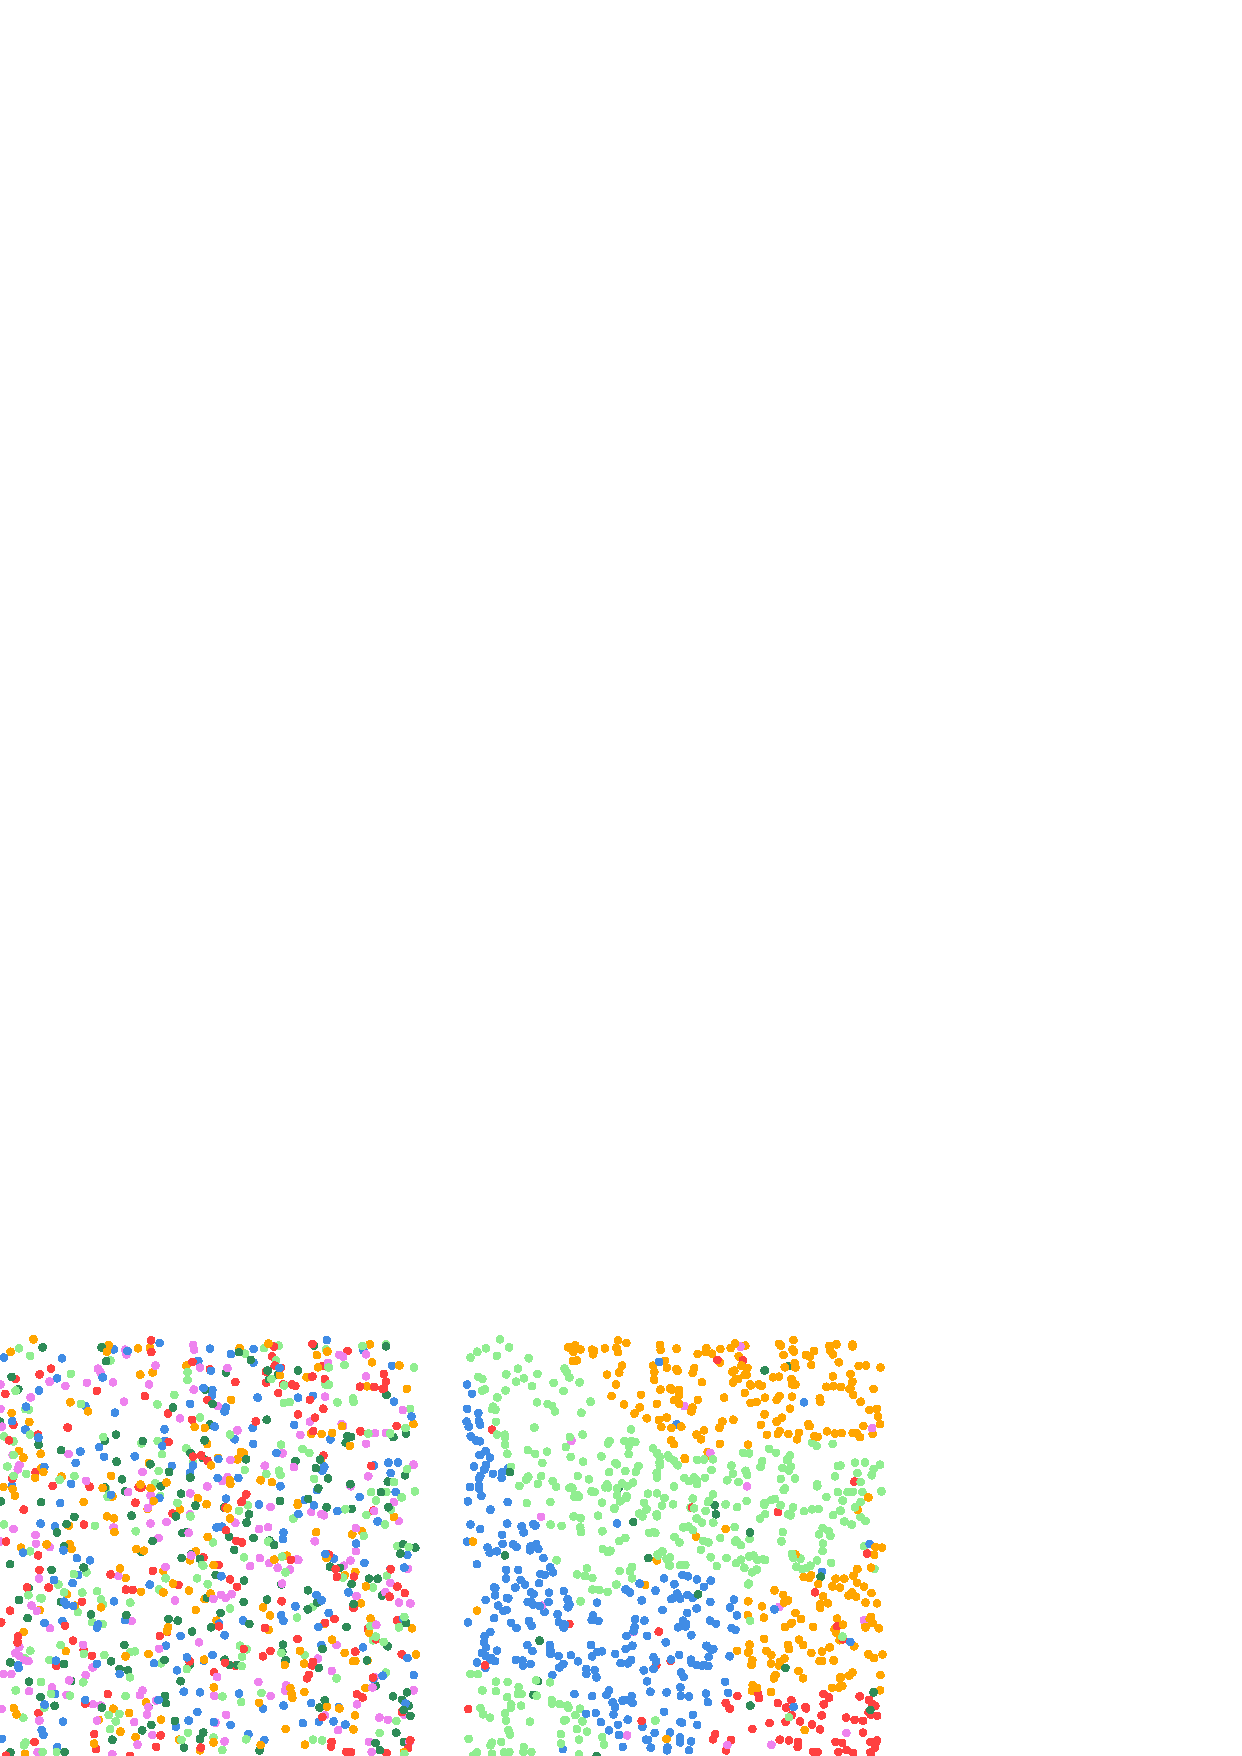
\includegraphics[width=\linewidth]{figures/groupedVsUniform}
   \caption{Left: a set of $\num{10000}$ points with $6$ uniformly random colors. Right: a set of $\num{1000}$ points with grouped colors, with $\alpha = 0.9$ and $\gamma = 10$. }
   \label{fig:groupedVsUniform}
\end{figure}


\begin{figure}[h]
  \centering
     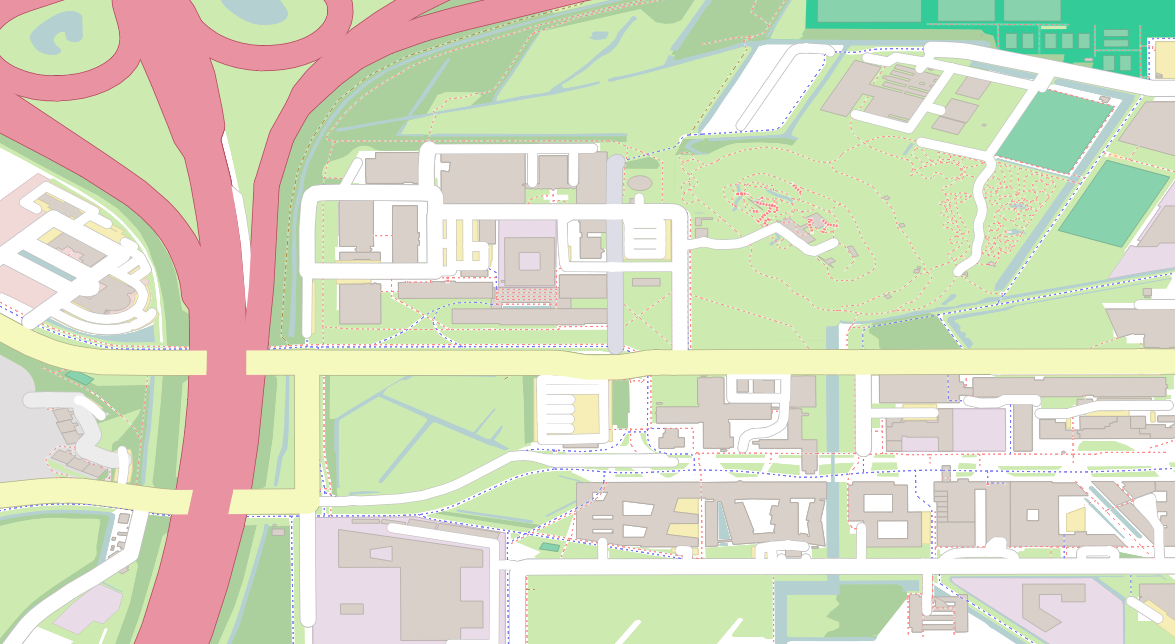
\includegraphics[width=.9\linewidth]{figures/usp.png}

     \vspace{10px}

    
\includegraphics[width=.9\linewidth]{figures/bbg}
   \caption{A map colored by terrain-type, then discretized (the actual colors after discretization are randomized).}
   \label{fig:usp}
\end{figure}

The set of experiments run in 1D is shown in \cref{tab:exp1D}, and in 2D is shown in \cref{tab:exp2D}. For each scenario we
build every datastructure from \cref{sub:implementedDatastructs} (when
applicable). Since the \cutting{} structure turned out to be significantly slower than
the others, we use values of $n$, $\phi$, $s$, and $\gamma$ that are up to $10$ times lower than for the other structures.




\begin{table*}[h]
\centering
\begin{tabular}{llllll}
\toprule
Experiment                            & $n$              & $\phi$      & $s$        & $\gamma$  & $\alpha$  \\
\midrule
Uniform data with increasing $n$      & \num{25000} - \num{300000} & \num{25000}      & $\sqrt{n}$ & -         & -         \\
Uniform data with increasing $\phi$   & \num{200000}          & \num{1} - \num{200000} & $\sqrt{n}$ & -         & -         \\
Uniform data with increasing $s$      & \num{200000}          & \num{25000}      & \num{2} - \num{1000}   & -         & 0 - 1     \\
Grouped data with increasing $\alpha$ & \num{200000}          & \num{25000}      & $\sqrt{n}$ & \num{10000}    & -         \\
\bottomrule
\end{tabular}
\caption{The parameters for the 1D experiments.}
\label{tab:exp1D}
\end{table*}

\begin{table*}[h]
\centering
\begin{tabular}{llllll}
\toprule
Experiment                            & $n$               & $\phi$      & $s$        & $\gamma$ & $\alpha$  \\
\midrule
Uniform data with increasing $n$      & \num{10000} - \num{150000}  & \num{10000}      & $\sqrt{n}$ & -        & -         \\
Uniform data with increasing $\phi$   & \num{100000}           & \num{1} - \num{100000} & $\sqrt{n}$ & -        & -         \\
Uniform data with increasing $s$      & \num{100000}           & \num{10000}      & \num{2} - \num{1000}   & -        & -         \\
Grouped data with increasing $\alpha$ & \num{100000}           & \num{10000}      & $\sqrt{n}$ & \num{5000}    & \num{0}-\num{1}       \\
%Real data: \texttt{OpenML}                    & \num{20000} - \num{120000}  & \num{22}          & $\sqrt{n}$ & -        & -         \\
Real data: \texttt{OSM}                       & \num{5000} - \num{8000}  & \num{10}            & $\sqrt{n}$ & -        & -         \\
\bottomrule
\end{tabular}
\caption{The parameters for the 2D experiments.}
\label{tab:exp2D}
\end{table*}


\subsection{Queries.}
A query is a square defined by a center point $c \in \R^2$, and a value
$k \in 1..n$ specifying its size (in the number of points that will be
in the query square). We use a fixed set of possible $k$ values,
ranging from $1$ to $n$. For each experiment and each value of $k$ we
produce $10000$ centers; for the synthetic datasets we generate these
uniformly at random (within the same bounds as the point set itself),
for the real datasets we randomly sample (and
remove) $10000$ points from the input point set. Given such a
center $c$ we then compute the smallest square centered at $c$ containing
exactly $k$ points using the range finding data structure, and then
compute a mode color using one of the mode finding data structures.




\section{Experimental results and analysis.}
\label{sec:Experimental_Results}
In this section we show the most interesting results of our
experiments, and analyze their meaning with respect to our research
questions. All results can be found along with the source code
in~\cite{code}. \erwin{and in appendix?}

\subsection{Practicality of sublinear methods.}
Our first research question concerns how practical these sublinear methods are. We first compare the \cutting structure to the \grid and \blocks structures in 1D, and then compare the \grid method to the naive \report and \rangeTrees methods in both 1D and 2D. We then study the dependency of the different structures to the parameter $k$, and lastly consider the relative importance of the range finding query versus the mode finding query.

\subparagraph{Cuttings in practice.}  
See \cref{fig:1D_comparison}. The \grid structure outperforms the \cutting structure in query time by a around factor $2$, and in build time and space usage by around a factor $10$, despite having the same asymptotical bounds and essentially doing the same thing. This indicates that the simplicity of the \grid structure, i.e. avoiding to build an explicit 2D arrangement and a point-location structure on it, indeed provides improved performance. Anectotally but importantly, the \grid structure was also significantly simpler to implement than the \cutting structure.

The \blocks structure vastly outperforms all other methods in query time, most notably for high $k$ values. This shows that avoiding the range counting queries (and thus
dealing with each point in amortized constant time) indeed pays
off significantly. Unfortunately these specific techniques do not easily translate to
higher dimensions.

\begin{figure*}[h]
  \begin{minipage}{0.33\linewidth}
    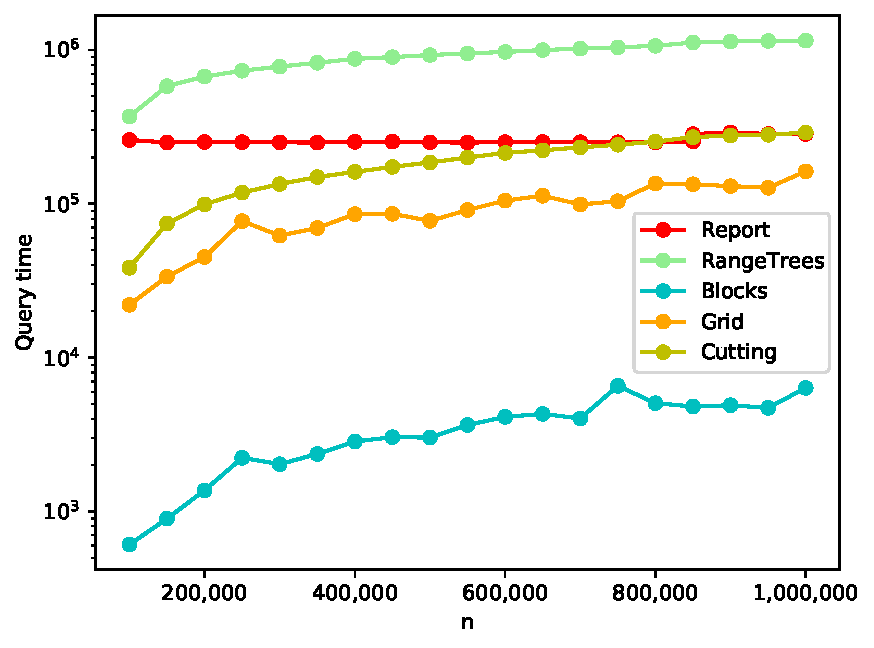
\includegraphics[width=\textwidth]{figures/graphs/1D_fullComparison_modeQueryTimeExcludingFirst.pdf}
  \end{minipage}%
  \hfill
  \begin{minipage}{0.33\linewidth}
    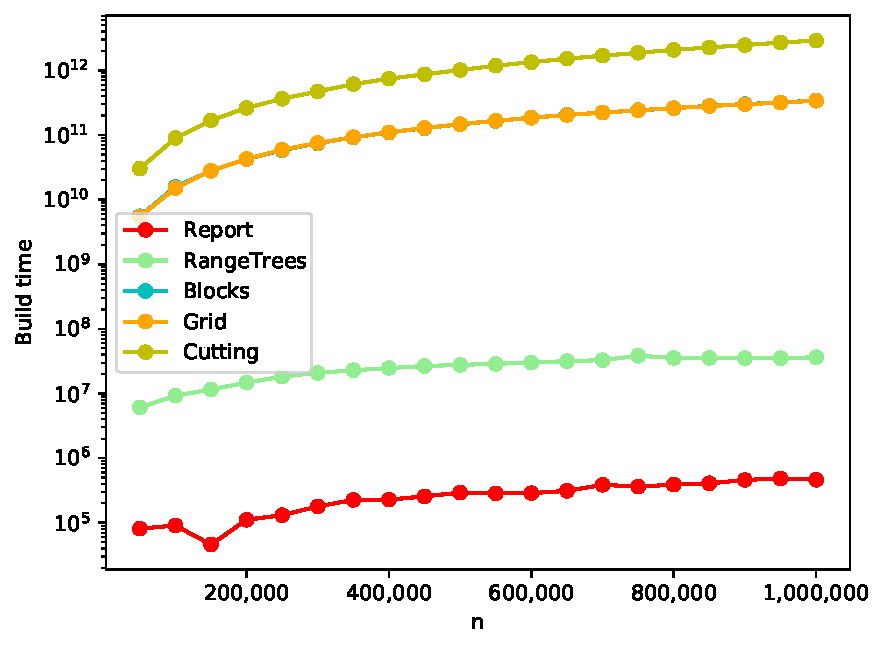
\includegraphics[width=\textwidth]{figures/graphs/1D_fullComparison_modeBuildTime.pdf}
  \end{minipage}%
  \hfill
  \begin{minipage}{0.33\linewidth}
    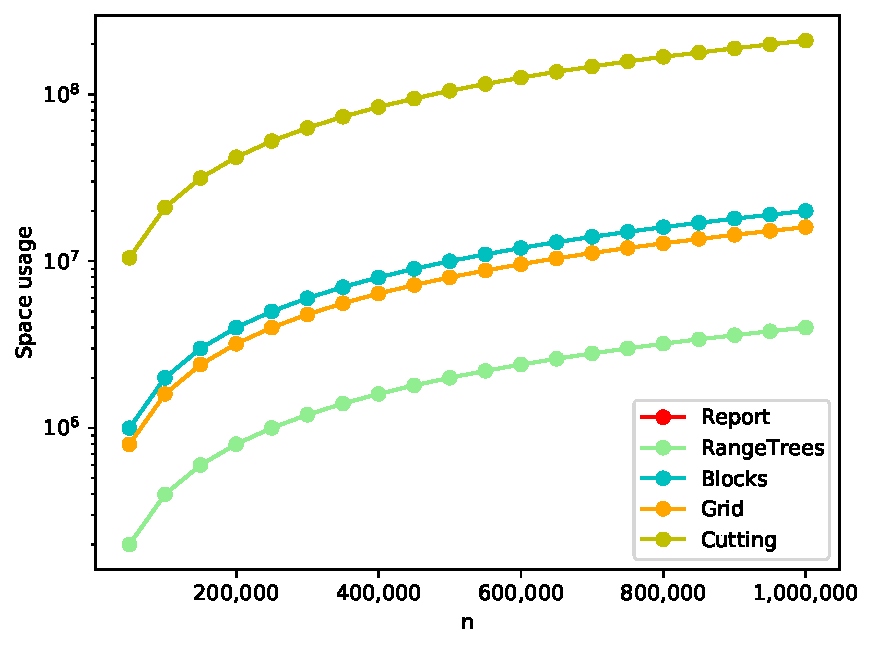
\includegraphics[width=\textwidth]{figures/graphs/1D_fullComparison_modeSpace.pdf}
  \end{minipage}%
\caption{Query time, build time, and space usage of the five 1D methods, using $k = \num{100000}$ and $\phi = \num{50000}$. }
\label{fig:1D_comparison}
\end{figure*}




\subparagraph{Comparing \grid and naive methods.}
See \cref{fig:1D_comparison} for the 1D results and \cref{fig:2D_comparison} for the 2D results. In both cases, for the chosen parameters, the \grid structure has a lower query time than both the \report and the \rangeTrees structures, showing that the more complicated sub-linear methods can indeed provide better performance than the naive methods, while using slightly more space and significantly more build time. 

Take for example $n = \num{500000}$ in 2D, where the \grid structure has around query time $\num{4}$ ms and build time $\num{900000}$ ms, while the \rangeTrees structure has around query time $\num{20}$ ms and build time $\num{300}$ ms. This means that, at these parameters, the \grid structure will start outperforming the \rangeTrees structure from around $\num{50000}$ queries, or only around $10\%$ of the number of points.



\begin{figure*}[h]
  \begin{minipage}{0.49\linewidth}
  \begin{minipage}{0.5\linewidth}
    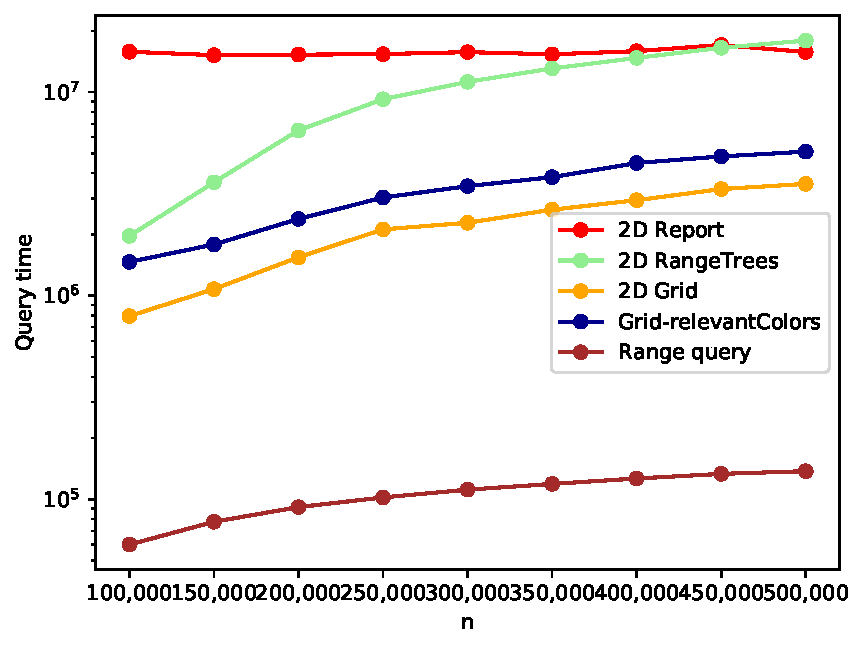
\includegraphics[width=\textwidth]{figures/graphs/2D_fullComparison_modeQueryTimeExcludingFirst.pdf}
  \end{minipage}%
  \hfill
  \begin{minipage}{0.5\linewidth}
    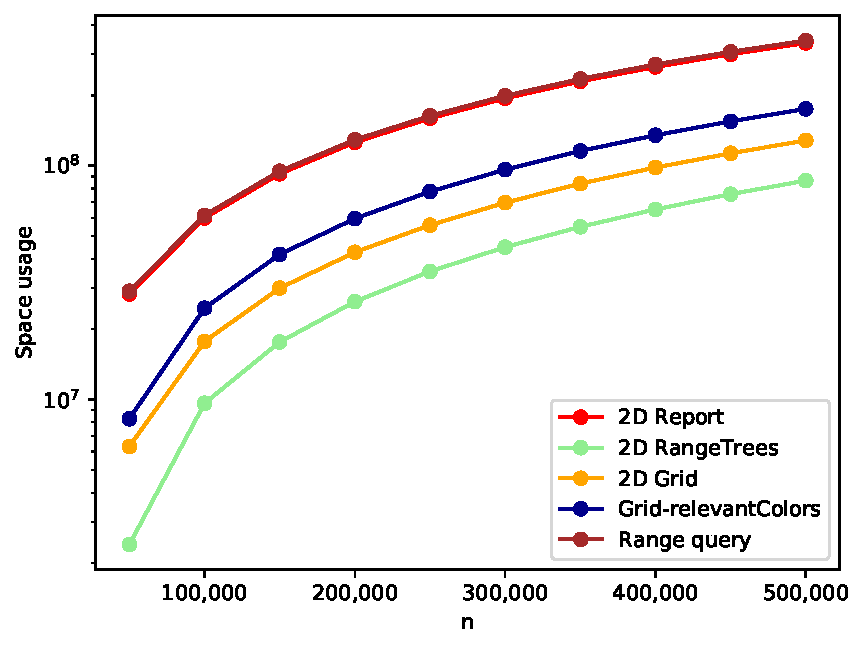
\includegraphics[width=\textwidth]{figures/graphs/2D_fullComparison_modeSpace.pdf}
  \end{minipage}%
  \caption{Query time and space usage for the 2D structures and the range-finding structure, using $k = \num{100000}$ and $\phi = \num{50000}$. }
\label{fig:2D_comparison}
  \end{minipage}%
  \hfill
  \begin{minipage}{0.49\linewidth}
  \begin{minipage}{0.5\linewidth}
    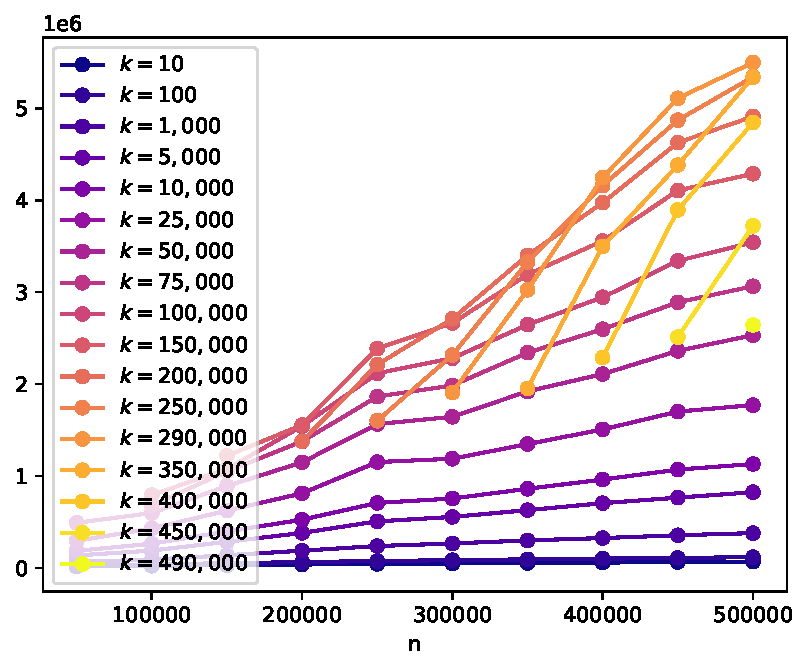
\includegraphics[width=\linewidth]{figures/graphs/2D_fullGridDetail.pdf}
  \end{minipage}%
  \hfill
  \begin{minipage}{0.5\linewidth}
    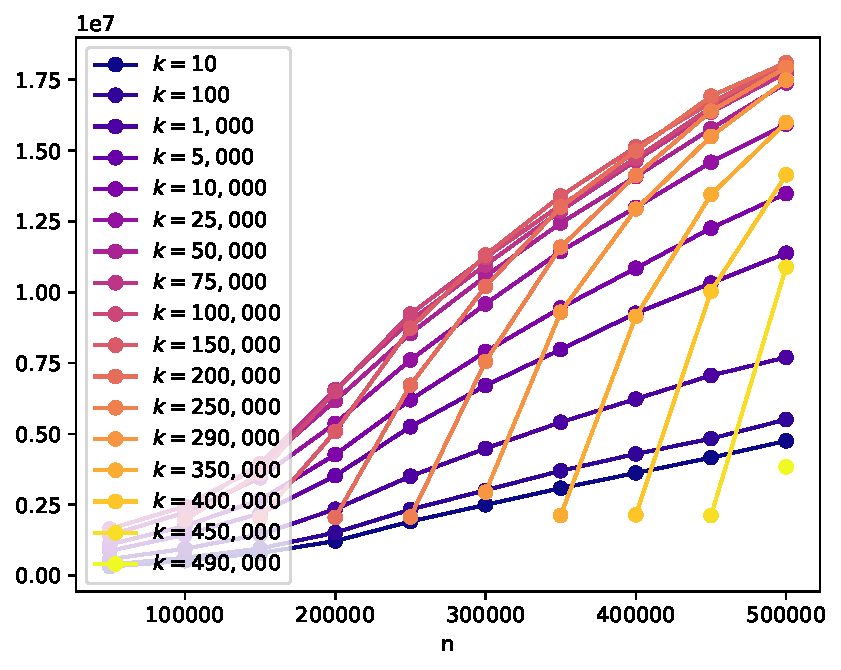
\includegraphics[width=\linewidth]{figures/graphs/2D_fullRangeTreesDetail.pdf}
  \end{minipage}%
  \caption{Query time \grid structure (left) and the \rangeTrees structure (right) for varying $k$ values, using $\phi = \num{50000}$.}
\label{fig:2D_detail}
  \end{minipage}%
\end{figure*}


\subparagraph{(In)dependence of $k$} 
One of the main theoretical
motivations behind the design of the \blocks, \cutting, and \grid
structures was to have a query time independent of $k$ and $\phi$, in
contrast to the simple \report and \rangeTrees structures. Although it
is true that the asymptotic worst-case upper bound is independent of
$k$, in practice some dependency remains visible for the \grid structure. See \cref{fig:kDependency,fig:2D_detail}. The smaller the value of $k$, the fewer points a query $q$ contains, and thus the fewer colors in the slabs containing $q$'s cornerpoints are contained in $q$. This results in fewer range-searches to be done, and thus a lower query time. 

For $k$ close to $n$ ($k > \num{350000}$ in \cref{fig:kDependency}) the query time starts decreasing as $k$ increases. This behaviour can be seen more strongly for the \rangeTrees structure. This is because very large queries are likely to contain all points of a color, in which case a query is answered much more quickly, both due to having a smaller set of canonical nodes and due to caching.

\begin{figure*}[h]
    \begin{minipage}{0.32\linewidth}
      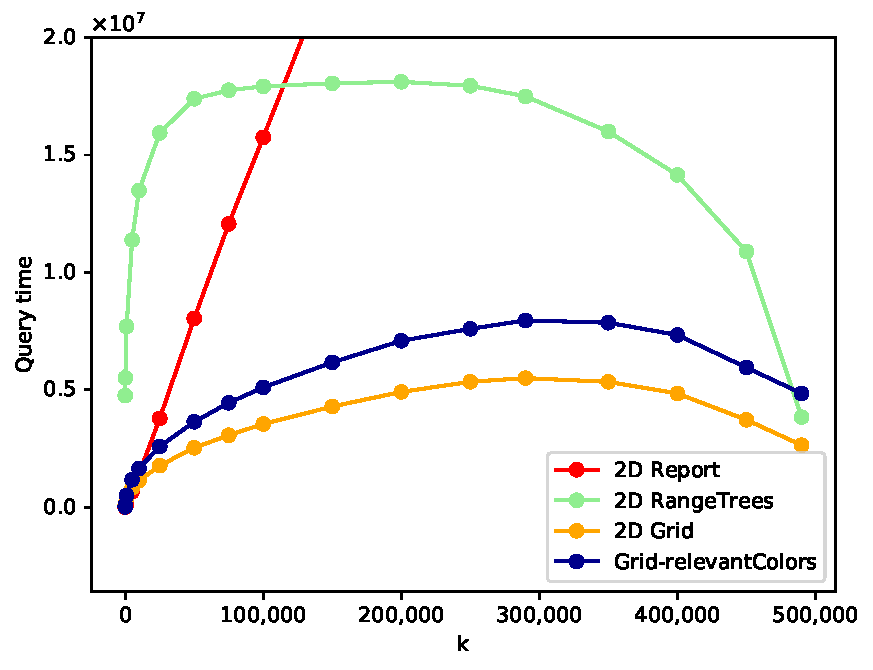
\includegraphics[width=\linewidth]{figures/graphs/2D_k_dependency.pdf}
      \caption{Query time of the \grid structure as a function of $k$, using $n = \num{500000}$ and $\phi = \num{50000}$. The \report graph is simply a straight line, and has been cut.}
      \label{fig:kDependency}
    \end{minipage}%
    \hfill
    \begin{minipage}{0.64\linewidth}
    \begin{minipage}{0.49\linewidth}
      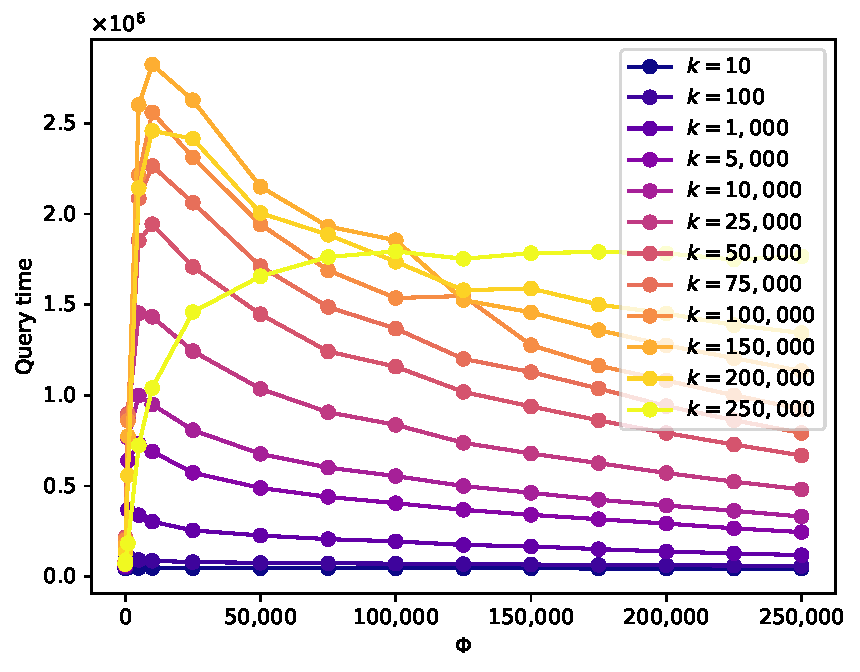
\includegraphics[width=\textwidth]{figures/graphs/2D_phiDependency_AAS2DModeGridDS.pdf}
    \end{minipage}%
  \hfill
  \begin{minipage}{0.49\linewidth}
    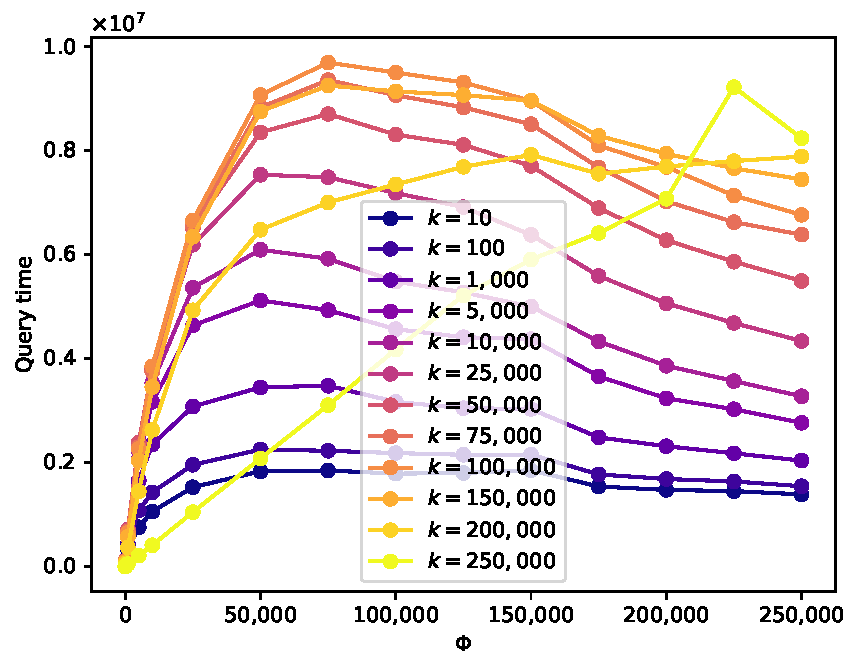
\includegraphics[width=\textwidth]{figures/graphs/2D_phiDependency_AAS2DModePerColorDS.pdf}
  \end{minipage}%
  \caption{Query time of the \grid structure (left) and the \rangeTrees structure (right) as a function of $\phi$, using $n = \num{250000}$.}
  \label{fig:phiDependency}
  \end{minipage}%
\end{figure*}

\begin{figure*}[h]
    \begin{minipage}{0.32\linewidth}
      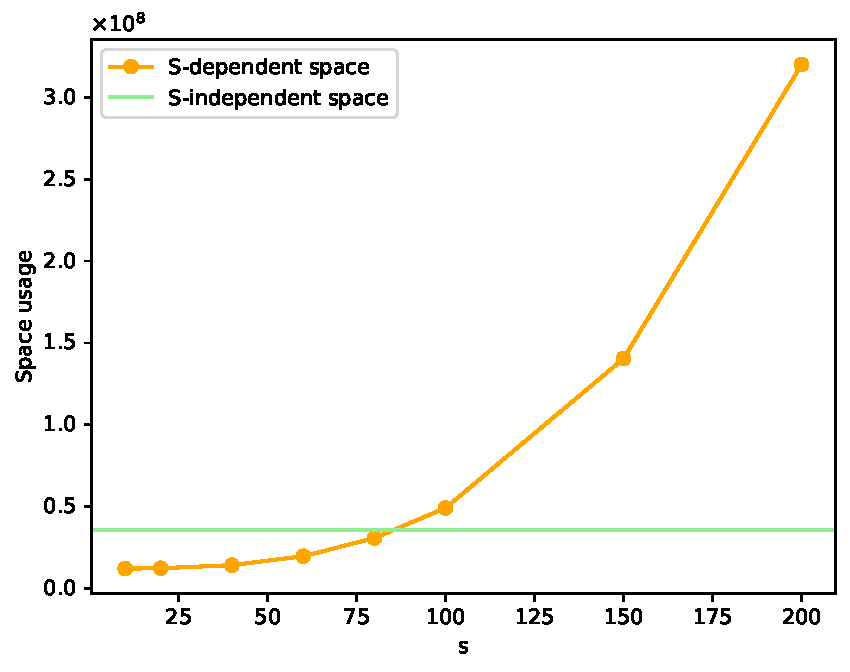
\includegraphics[width=\textwidth]{figures/graphs/2D_sDependency.pdf}
      \caption{Space usage of the \grid structure as a function of $s$, using $n = \num{250000}$ and $\phi = \num{50000}$, split into $s$-dependent and $s$-independent space.}
      \label{fig:sDependency}
    \end{minipage}%
    \hfill
    \begin{minipage}{0.64\linewidth}
    \begin{minipage}{0.49\linewidth}
      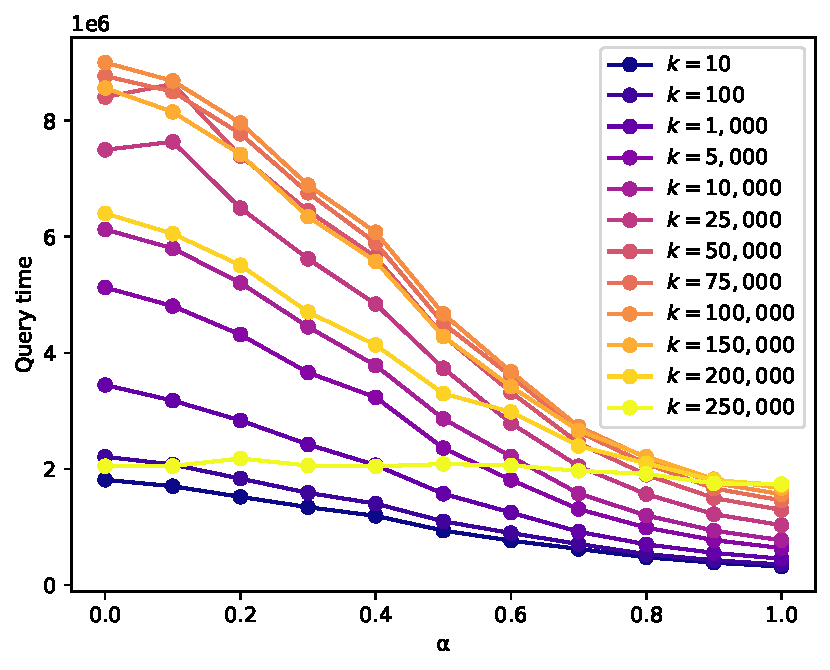
\includegraphics[width=\textwidth]{figures/graphs/2D_alphaDependency_AAS2DModePerColorDS.pdf}
    \end{minipage}%
  \hfill
  \begin{minipage}{0.49\linewidth}
    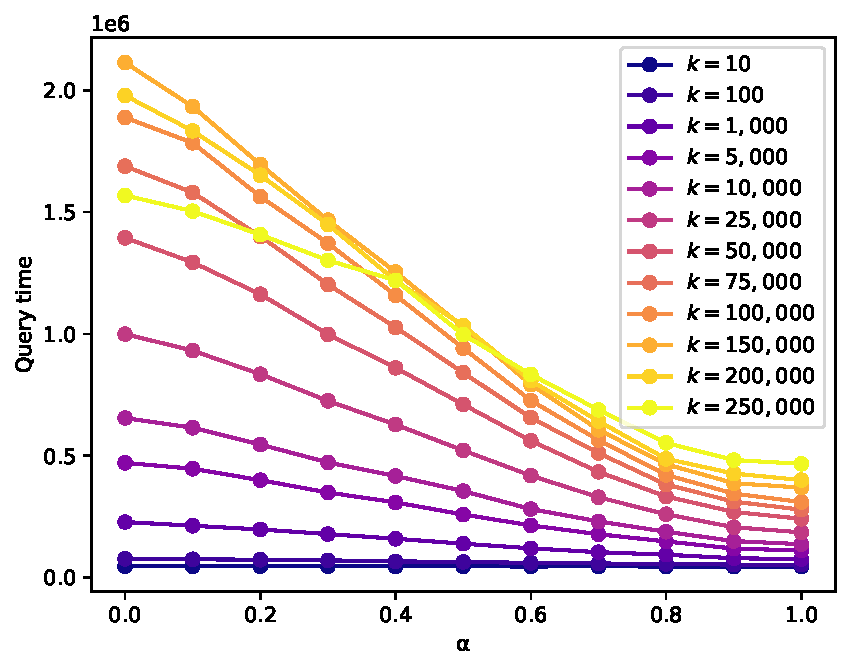
\includegraphics[width=\textwidth]{figures/graphs/2D_alphaDependency_AAS2DModeGridDS.pdf}
  \end{minipage}%
    \caption{Query time of the \grid structure (left) and the \rangeTrees structure (right) as a function of $\alpha$, using $n = \num{250000}$ and $\phi = \num{50000}$.}
    \label{fig:alphaDependency}
  \end{minipage}%
\end{figure*}



\subparagraph{Ratio between range-finding and mode-finding}
Our main focus has been on the different structures for mode-finding queries given a square, but to answer a $k$NN query we first need to actually find this square using a range-finding structure. See \cref{fig:2D_comparison}. The range query contributes only a small portion of the total query time, being at least $10$ times as fast as all mode-finding structures. This indicates that, both in theory and in practice, the mode-finding portion of the problem requires significantly more time, and is thus more interesting to optimize.




\subsection{Parameter choice.}
Our second research question considers the practical influence of the user-set parameter $s$.
See \cref{fig:sDependency}, where $n = \num{100000}$ and $\phi = \num{1000}$ ($n = \num{10000}$ and $\phi = \num{100}$ for the \cutting structure). In the figure we separated the $s$-dependent space usage (most importantly the \texttt{blockModes} table) from the $s$-independent space usage (the range trees).

Theory tells us we should choose $s = O(n^{1/{d+1}})$ for a good
tradeoff between (linear) space and (sub-linear) query time, but this
leaves us free to choose a constant ($s = \frac{n^{1/{d+1}}}{10}$ vs
$s = 10 n^{1/{d+1}}$). A logical choice would be to choose $s$ such
that the space usage dependent on $s$ is about equal to the space
usage independent from $s$, to obtain a good query time without sacrificing too much extra space. From our experiments, this is somewhere between $s = 75$ and $s = 100$, which is
quite close to the theoretical value $s = n^{1/{d+1}} = 63$. This indicates that the choice of $s = n^{1/{d+1}}$ indeed provides a good practical tradeoff between query time and space usage.




\subsection{Dependency on data distribution.}
Our last research question considers the dependency of the \grid structure on the color distribution of the data. We compare the performance on uniform random point sets with varying numbers of total colors $\phi$, on uniform random point sets with varying level of groupedness $\alpha$, and on real datasets.


\subparagraph{Varying $\phi$.} See \cref{fig:phiDependency}. The query times are very fast for very low values of $\phi$, since the query time is mainly dominated by the number of counting queries that must be done; if there are only few colors, we must only perform few counting queries. As $\phi$ grows larger we see a slight decrease in query time, since the number of points per color decreases, and thus each individual counting query becomes faster. Similar behavior can be observed in the \rangeTrees structure. The effect is more pronounced for the \grid structure since it does at most $O(n/s)$ counting queries, rather than $\phi$ counting queries for the \rangeTrees structure.

\subparagraph{Varying $\alpha$.} See \cref{fig:alphaDependency}. As $\alpha$ increases, the query time decreases significantly. This is likely partially because there are fewer different colors in each strip and we thus collect a smaller set of colors for which we have to perform counting queries. However, similar behavior can again be observed in the \rangeTrees structure. This might be because, if a color is very strongly grouped, many queries contain the same subset of points, for example containing all points of that color or none at all, increasing cache-effectiveness. In contrast, if a color is distributed uniformly, it is much less likely that two queries contain the same points of that color.

\subparagraph{Real datasets.} See \cref{fig:realData}, and note that these datasets use only $\phi = 11$ colors, and thus all structures have relatively low query time for reasons discussed above. The performance on all three datasets is nearly identical for all values of $n$ and $k$, indicating that with so few colors, it does not make much difference whether they are grouped realistically, grouped synthetically, or colored uniformly at random.
 

\begin{figure*}[h]
  \begin{minipage}{0.33\linewidth}
    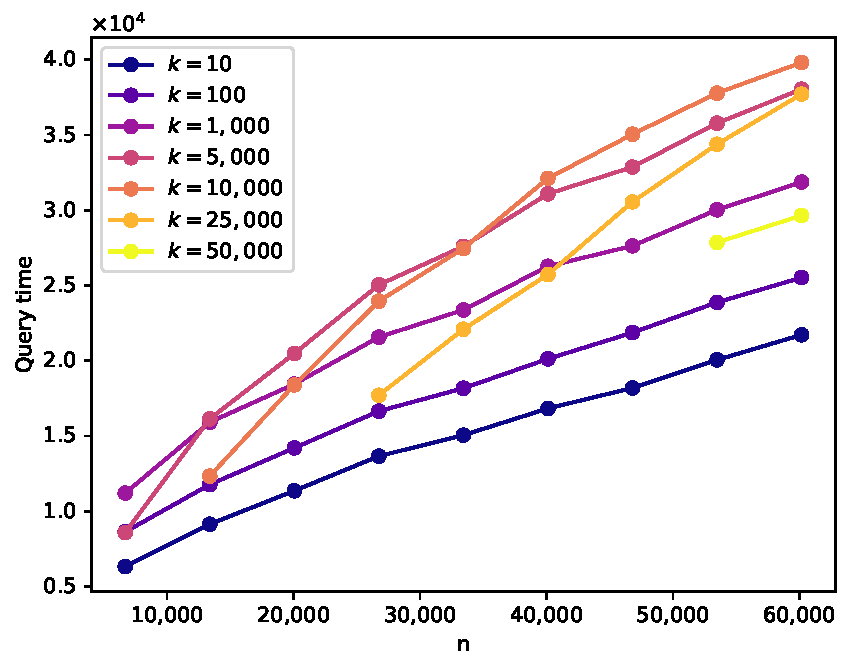
\includegraphics[width=\textwidth]{figures/graphs/2D_bbg.pdf}
  \end{minipage}%
  \hfill
  \begin{minipage}{0.33\linewidth}
    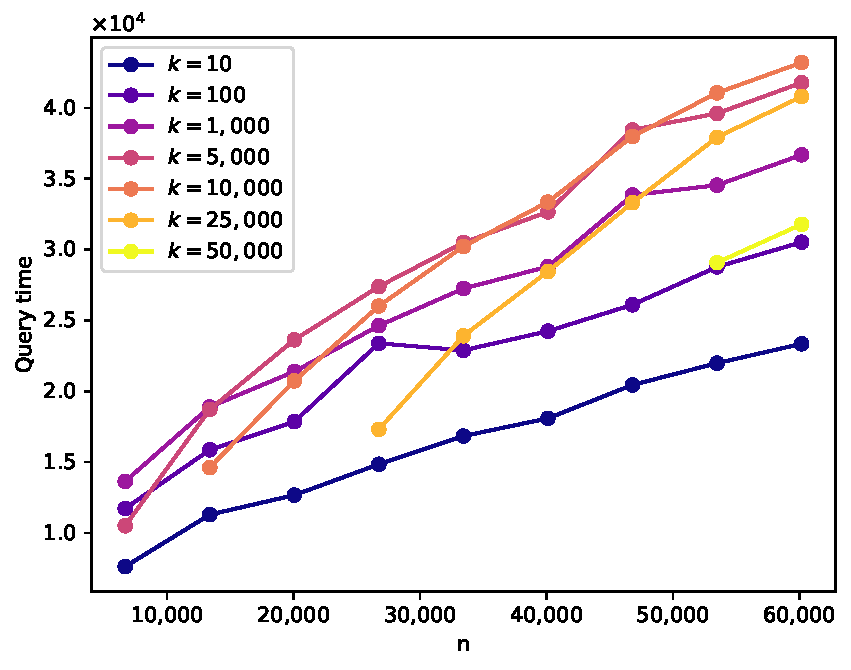
\includegraphics[width=\textwidth]{figures/graphs/2D_bbgSynthetic.pdf}
  \end{minipage}%
  \hfill
    \begin{minipage}{0.33\linewidth}
    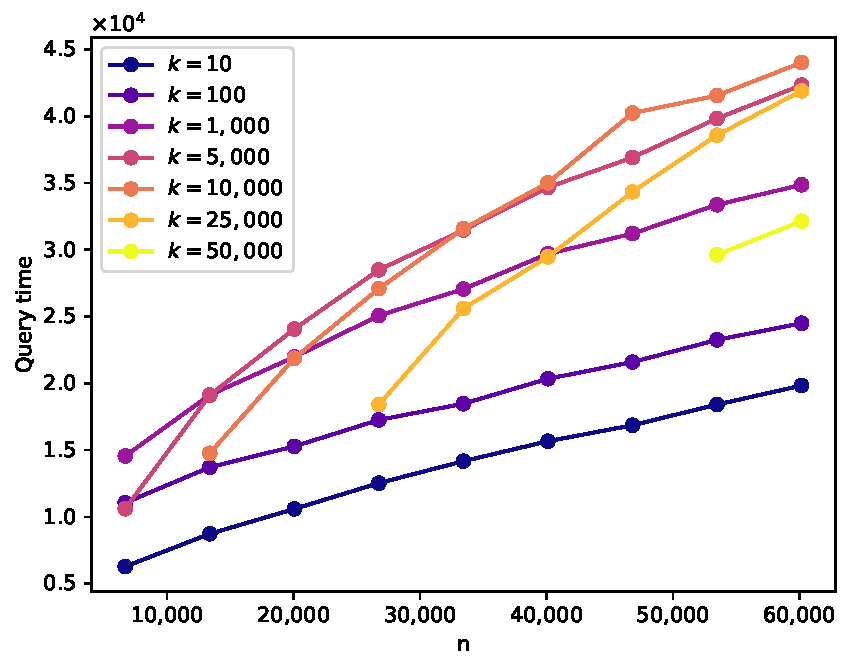
\includegraphics[width=\textwidth]{figures/graphs/2D_bbgSyntheticGrouped.pdf}
  \end{minipage}%
\caption{Query time of the \grid structure in 2D on subsets of a real dataset (OSM-bbg) with $n = \num{66870}$ and $\phi = 11$ (left), and on synthetic datasets with uniform random colors (middle), and on synthetic datasets with grouped colors with $\alpha = 1$ and $\gamma = \num{1000}$ (right).}
\label{fig:realData}
\end{figure*}







\section{Concluding remarks.}

In this article we implemented and compared several different data
structures for mode finding queries. We found that our simplified
\grid structure performed better than the \cutting structure in 1D,
despite having equal worst-case asymptotic lower bounds, indicating that it may be worthwhile to strive for simplicity in algorithm design, both for ease of understanding and for performance reasons. Both in 1D and in 2D the \grid structures could also outperform the naive \rangeTrees and \report structures, for certain parameters $\phi$ and $k$, already for a modest number of queries. Secondly, the dependency on the parameter $s$ was as we
would expect. Lastly, the \grid structures was relatively consistent
across different color distributions in the input set; performing slightly better on datasets with very few or very many colors and on datasets with highly grouped colors. \erwin{nog iets van algemene conclusie? weet niet precies wat}

\subparagraph{Future work.} In this article we focused on the
$L_\infty$ distance measured, and showed that we could use its
geometric properties to significantly simplify the cutting-based mode
finding data structure. Our results extend to other polyonal distance
functions (such as $L_1$). The cutting based approach works for even
more general distance measures (e.g. $L_2$ as well). An interesting
question is if a similar simplifications are applicable in that
setting as well. Furthermore, how does this more general method
perform in practice?


\bibliographystyle{siamplain}
\bibliography{bibliography}


\clearpage



\section{Omitted Proofs.}
\label{app:Omitted_Proofs}

\gridforCubes*

\begin{proof}
  The unit disk in the $\hat{L}$ metric is the intersection of some constant
  number $c$ of $d$-dimensional halfspaces, bounded by
  $(d-1)$-dimensional hyperplanes $h_1 \ldots h_c$.

  Consider one hyperplane $h_i$ of the unit polytope. We sort the points in the direction of its normal, and partition space into $s$ strips using $s$ $(d-1)$-dimensional hyperplanes paralel to $h_i$, each strip containing $O(n/s)$ points. Doing this for all $c$ polytope hyperplanes $h_i$ results in a set $H$ of $O(s)$ strip-hyperplanes in total (recall $c$ is a constant), forming a non-standard grid, as in \cref{fig:constantComplexityUnitDisk}. Given a query $Q$ we can once again find the span, the largest sub-grid that is fully contained in $Q$, of which we wish to know the mode color. There are $O(s^c)$ such distinct possible spans, since there are $O(s)$ strips in all $c$ directions. We once again show that there are only $O(s^{d+1})$ distinct spans that correspond to actual queries. The rest of the data structure remains the same; after finding the mode of a span we iterate through all remaining points in the strips containing the sides of $Q$.

  Consider again the parameter space $\R^{d+1}$ where each point $(x,r) \in \R^{d+1}$ corresponds to a query centered at $x \in \R^d$ with radius $r \in \R$, i.e. the unit polytope scaled by a factor $r$. Consider the unit polytope at height $r=1$ centered at the origin, and for each $d$-dimensional halfspace bounded by $(d-1)$-dimensional hyperplane $h_i$ that the polytope consists of, consider the $(d+1)$-dimensional halfspace bounded by $d$-dimensional hyperplane $h'_i$ that goes through it and through the origin. The intersection of these halfspaces $h'_i$ is exactly the set of points $(x,r)$ corresponding to a query centered at $x$ with radius $r$ that contains the origin. This is analogous to the upside-down pyramid from \cref{fig:thijsMethodPyramid}, where the unit polytope is a square.

  For each $(d-1)$ dimensional grid-hyperplane in $H$ we create the $d$-dimensional hyperplane through it that is paralel to $h'_i$. These $O(s)$ hyperplanes partition $\R^{d+1}$ into $O(s^{d+1})$ cells. As before, all $(d+1)$-dimensional points within one cell of the arrangement are indistinguishable w.r.t. the $d$-dimensional hyperplanes. That means their corresponding queries intersect the same grid-hyperplanes from $H$, and thus have the same span.  It follows that there are only $O(s^{d+1})$ distinct spans that correspond to actual queries in the grid. Precomputation of these spans remains the same, by traversing the above arrangement (implicitly).
\end{proof}


\end{document}